%% $RCSfile: proj_report_outline.tex,v $
%% $Revision: 1.3 $
%% $Date: 2016/06/10 03:41:54 $
%% $Author: kevin $

\documentclass[11pt
              , a4paper
              , oneside
              ]{report}


\usepackage{float} % lets you have non-floating floats
\usepackage{url} % for typesetting urls
\usepackage[image,ecs]{vuwproject}
\usepackage{booktabs}
\usepackage[table,xcdraw]{xcolor}
\usepackage{wrapfig}
\usepackage{lscape}
\usepackage{graphicx}
\usepackage{wrapfig}
\usepackage{lipsum}
% \usepackage[
%     backend=biber,
%     style=alphabetic,
%     sorting=ynt
%     ]{biblatex}
    
\usepackage[english]{babel}
\usepackage[style=ieee,backend=bibtex]{biblatex}
\addbibresource{sample.bib}

%
%
%  We don't want figures to float so we define
%
\newfloat{fig}{thp}{lof}[chapter]
\floatname{fig}{Figure}

%% These are standard LaTeX definitions for the document
%%                            
\title{Automated Essay Scoring Using Machine Learning with Manual Feature Engineering And Regression Models
}
\author{James Ian Rowles}

%% This file can be used for creating a wide range of reports
%%  across various Schools
%%
%% Set up some things, mostly for the front page, for your specific document
%
% Current options are:
% [ecs|msor|sms]          Which school you are in.
%                         (msor option retained for reproducing old data)
% [bschonscomp|mcompsci]  Which degree you are doing
%                          You can also specify any other degree by name
%                          (see below)
% [font|image]            Use a font or an image for the VUW logo
%                          The font option will only work on ECS systems
%

% 

\supervisors{Sharon Gao }

% You should specifiy your supervisor here with
%     \supervisor{Firstname Lastname}
% use \supervisors if there is more than one supervisor

\otherdegree{Bachelor of Engineering with Honours}

% Unless you've used the bschonscomp or mcompsci
%  options above use
%   \otherdegree{OTHER DEGREE OR DIPLOMA NAME}
% here to specify degree

% Comment this out if you want the date printed.
\date{}


\begin{document}

% Make the page numbering roman, until after the contents, etc.
%\frontmatter

%%%%%%%%%%%%%%%%%%%%%%%%%%%%%%%%%%%%%%%%%%%%%%%%%%%%%%%

%%%%%%%%%%%%%%%%%%%%%%%%%%%%%%%%%%%%%%%%%%%%%%%%%%%%%%%

\begin{abstract}

The primary aim of this project is to grade students' essays from The English Proficiency Program automatically. This research aims to address this issue by examining an approach using regression models and feature engineering.

\end{abstract}

%%%%%%%%%%%%%%%%%%%%%%%%%%%%%%%%%%%%%%%%%%%%%%%%%%%%%%%

\maketitle

\tableofcontents

%%%%%%%%%%%%%%%%%%%%%%%%%%%%%%%%%%%%%%%%%%%%%%%%%%%%%%%

\mainmatter

%%%%%%%%%%%%%%%%%%%%%%%%%%%%%%%%%%%%%%%%%%%%%%%%%%%%%%%

% individual chapters included here
\paragraph{Acknowledgements}
I want to thank my supervisors Sharon Gao and Peter Gu for their support and guidance throughout this project. I would also like to express my gratitude towards my supervisors for providing me with this opportunity. As an individual who highly values the pursuit of learning and has played both roles - teacher and student. I feel very privileged to be given the opportunity to contribute back to this community. Lastly, I would like to thank my examiners for their contribution to completing this project.

\backmatter

\chapter{Introduction}\label{C:intro}

\section{Context}

Hundreds of students take the English Proficiency Programme (EPP) every year. Its aim is to help students develop their English in a welcoming learning setting. In addition, the EPP can train a pupil for more English-language academic training. The EPP facilitates a test to assess a student's ability to see if they would meet the entry criteria for their specific undergraduate or postgraduate course. This test consists of multiple components, including a multi-choice and a writing component. Based on how they perform overall dictates whether or not they will enter their proposed course [1]. However, if their overall performance is unsatisfactory, they will stay with the EEP to build their skills. In this case, it is beneficial for the academic staff of the EPP to understand which areas the student is struggling in to provide more tailored support for that student. 

\section{Problem}

The problem that exists here is that manually marking the writing component of this test takes too long and, as a result, is not included when making the final decision regarding whether or not a student has met their respective course's entry criteria. Excluding this component means that students are potentially not assessed as accurately as they could be. As a result,they can not receive the most optimal academic experience.

\section{Purpose}

The purpose of this project is to create a system that can automate this task.
Roughly, this looks like a system that can use an essay as input and, in return, provide quantifiable metrics regarding the essay's use of the English written language. 

\section{Goals}

The goals for the solution are for it to be relatively fast, precise enough, and easy to use and understand. 
\paragraph{Speed}
As speed is a leading contributor to the problem, this plays a massive part in the goals of the solution. Specifically, this means that it must be faster than if a human marker were doing it. 

\paragraph{Accuracy}
We need the system to predict similar marks to what a human rater might produce in terms of accuracy. However, as mentioned previously, the writing component is not used currently due to time constraints. As a result, even if the system were roughly accurate, it would still provide valuable insight to the academic staff. For example, its results could be used "with a grain of salt" and in combination with other assessment metrics at the final-judgment stage of the EPP program.

\paragraph{Easy of Use}
In terms of ease of use, for the final product, this may be defined as having a polished user experience held together with simple, maintainable network architecture. For this project's scope, I want to prioritize keeping the system explainable or understandable so that non-technical stakeholders have insight into the nature of the system - how it works, why it does things. Additionally, I want the system to be easily understood by a technical stakeholder such as the next student to work on this project. 

\section{Approach}

Initially, we saw there being two approaches to the problem. 

\paragraph{Approach 1} The first approach would provide a binary output to indicate whether the student had a good enough proficiency to enter their proposed university course or needed to continue with the EPP to improve their English writing proficiency further.

\paragraph{Approach 2}
The second approach would aim to go a step further by providing a continuous output that would provide insight into the extent of a student's overall writing proficiency and their categorical proficiency in areas such as; grammar, vocab, or ideas. With this approach, not only do we receive enough information to assess if they can enter their proposed university course or not. We can also go a step further by having insight into the extent to which they may or may not do so. For example, if the student needs to get an overall score of 4 to progress and receive a 3, this might lead us to believe that maybe they are not ready to progress. Also, with this approach, we get the same continuous-type output for specific categories. This means that, for the students who do not progress, we have insight into the areas that a student may be struggling with and the extent to which they may be struggling with them. This, then, allows for more tailed academic support. The same goes for areas that a student might be proficient in. 

\paragraph{}The latter provides the most information and consequently the most benefit for all stakeholders. So right from the offset, this was the approach that I wanted to take, provided it was a feasible pursuit.
\chapter{Background}\label{C:back}

To investigate the feasibility and potential pathways, I started by looking into general applied machine learning practices and academic papers about already existing systems like the one I was pursuing. Not to my surprise, I found that this process of automating essay scoring has been a subject of study for a while, specifically within education and business. An early note-able pursuit within this field dates back to the 1960s where Ellis Batten Page's PEG, Project Essay Scorer, began to gain public and scientific momentum and acceptance [2]. The systems that are products of this area are called AES's - Automatic Essay Scorers. A good AES can deliver scores that are relatively similar to human ratings. For example, the Educational Testing Service's e-rater system, also known as "e-rater," can produce accurate results over 90$\%$ percent of the time [3]. 

\section{Machine Learning}

AES systems have incorporated a sub-field of Artificial intelligence, Machine Learning, from early as 2013 [4]. Predictive Machine Learning is the science of making computers intelligent enough to make their own decisions. It has been around for a long time, but it has become powerful enough that it can now be used on various problems in recent years. Predictive Machine learning is generally used for tasks where it is beneficial for a computer to understand a relationship between an input and an output for a specific problem [5]. This is often used to use this relationship understanding to synthesize an output when only given an input. In our case, this relationship is between a text, and it is the corresponding score. We want to refine this relationship between the input and output to be given an unmarked essay and produce a score. 

\section{Models}

This relationship is called a model and is defined as a description of a system defined with mathematical concepts and language [6]. The model of an AES is a critical component of the overall solution. There are several types within the field of Machine Learning and AES. They can be divided into two categories. The first category consists of relatively simple models that employ statistical calculations such as Regression or Classification. Regression can be used to predict continuous values, for example, a score of "5.0" or "3.1" [7]. Classification can be used to identify, separate, or categorise values into discrete values, such as "true" or "false" [8]. The second category consists of relatively more complex models. These models work by simulating a network of interconnected nodes that work similarly to neurons in the human brain. To recognize and learn correlations within the data. They can then be used to predict continuous or discrete data [9].

\section{Feature Extraction}

Each model requires its input to be in a process-able format and descriptive of the problem before it can mathematically evaluate it. This process of optimizing the input to a more interpretable format is called Feature Extraction [10]]. When using a Neural Network model, this step can be skipped entirely [11]. However, when working with Regression and Classification models, this step must be performed manually using Manual Feature Engineering. This requires identifying and programmatically developing Features from an essay that are thought to indicate the skills being assessed [12. In our case, a feature can be thought of as a characteristic, property, or attribute of an essay. For example, the number of words in the text, the number of grammatical errors, or the average length of the words used. This process is done one feature at a time, requires domain knowledge, and can be time-consuming and error-prone. 

\section{Model Choice}

\paragraph{Prediction Type}
The output alone influenced my decision to deviate from a classification model. As, fundamentally, classification is about predicting a categorical variable. However, this type of output variable could be used to address the first approach mentioned in the introduction by, for example, classifying a student into either a "doing well" or "not doing well" group for a marking-criteria category. Neural and Regression models can do better by producing continuous outputs or predictions that align better with this project's preferred approach as they would produce a continuous output for a marking-criteria category.  

\paragraph{Nature of Relationship}
The nature of the relationship that is being investigated is also a crucial consideration. In some applications, neural network models can perform better than linear regression models when there are non-linearities involved. This is because neural networks, when appropriately configured, can understand highly complex and convoluted non-linear relationships. [13]. Non-linearity is a term used in statistics to describe a situation where there is no straight-line or direct relationship between two variables. In a non-linear relationship, changes in the output do not directly change to changes in any of the inputs [14]. In this study, I expect to observe linear relationships between the features and the output due to the nature of the problem of this project. I would expect to see that as the number of grammatical errors increases, the computer-generated score will decrease. This influenced my decision to lean toward a Regression model as they can perform well with linear relationships[x]. Additionally, they can do so with less configuration and, therefore, domain knowledge [x].

\paragraph{The Data}
The data available also plays a considerable role in narrowing down model options. As its size and relevance can influence a models' ability to synthesize the relationship in question. This is especially true for Neural Network models due to their better generalised ability to learn. As for where more data is available, better results can be observed from Neural network models [x]. However, in cases where this is not true, a Regression Model can be a better choice. For the duration of this project, nine datasets were used. Of these datasets, only one directly represented the problem and was not available for the entire duration of the project either. For these reasons, I saw a Regression Model being a better choice.

\paragraph{Feature Extraction}
Feature Extraction is another critical consideration when choosing a model. When considering a Neural model, the possibility of skipping the process of Manual Feature Engineering entirely can sound like an immediate win. However, despite Manual Feature Engineering introducing another component into the mix, it can provide much value. Especially when dealing with smaller datasets. Lilja observed a performance decrease in their study with Neural Models. And suggested that human insight when working with linguistic features could be crucial when dealing with small sample sizes [15]. Additionally, I'm optimistic about Manual Feature Engineering as I believe most features will not require extensive domain knowledge and are also relatively subjective. For these reasons, from the perspective of the available data, I saw value in Manual Feature Engineering. 

\paragraph{Explain-ability}
Lastly, explain-ability is an essential factor in this consideration as it aligns with the high-level goal of this project. Explainability is the concept that a machine learning model and its output can be explained in a way that "makes sense" to a human being at an acceptable level. When considering Manual Feature Engineering alone, there are already gains in explainability as the Feature Extraction step would be exposed and become the researchers' responsibility. This would mean that this step can be more easily explained to stakeholders. In addition, to provide insight, such as; what the features are and for which calculations they are being used for. Additionally, even without Manual Feature Engineering, Regression models are more accessible to explain than Neural Network models [x]. For these reasons, from the explaibabity, I saw a Regression with Manual Feature Engineering Model being a better choice.

\paragraph{}As discussed in the previous sections, Manual Feature Engineering paired with a Regression Model is the most optimal starting point for this project.

\chapter{Design}\label{C:des}

This project's scope is concerned with the development and experimentation of the two core components that make up this system. These are The Feature Extractor and The Predictor. Although this project is relatively immature, I have paid some respects to the theoretical end-solution at each project stage. This was important as it relates to the motivation behind the project - to provide the stakeholders with a usable tool. In saying this, the following diagram is a naive representation of the theoretical end-solution or product. 

\begin{figure}[h]
     \centering
     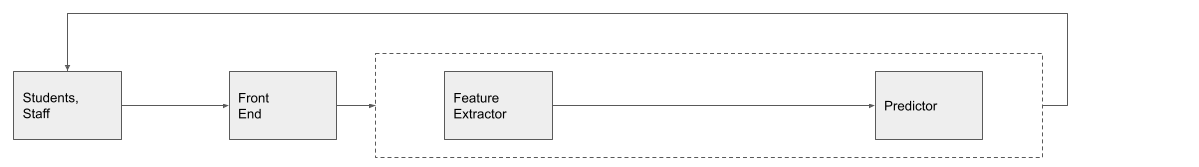
\includegraphics[width=.8\linewidth]{pngs/prod.png}
     \caption{AES as a Product}\label{Fig:Data1}
\end{figure}

As for the scope of this project, as mentioned previously, it is concerned with the development and experimentation of the Feature Extractor and The Predictor. Additionally, as with any machine learning endeavor, it heavily relies on relevant data to develop, test, and evaluate. Therefore, another critical in this investigation is The Prediction Configuration Generator (PCG). The PCG, paired with The Predictor and The Error Calculator, allowed for extensive exploration, insight, and evaluation of the system. 

\begin{figure}[h]
     \centering
     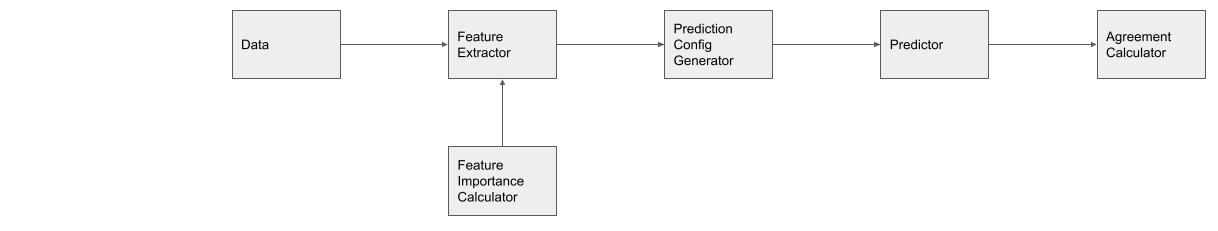
\includegraphics[width=.8\linewidth]{pngs/dev.png}
     \caption{AES in Development}\label{Fig:Data1}
\end{figure}

\section{The Data}
Preparing the data for the Feature Extractor can be broken down into three main stages - discovery, digitising, and processing. The product of these stages is the structured digital representation of an essay given to the Feature Extractor.

\begin{figure}[h]
     \centering
     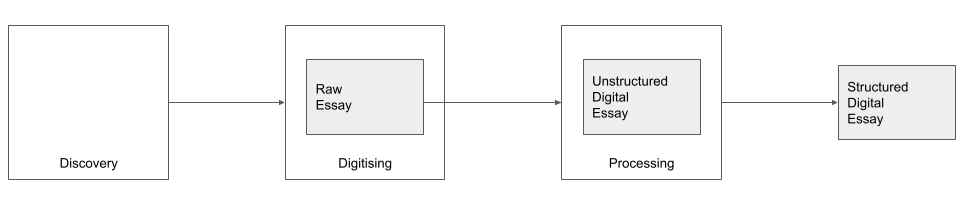
\includegraphics[width=.75\linewidth]{pngs/data-stages.png}
     \caption{The Data: Stages}\label{Fig:Data1}
\end{figure}

\subsection{Discovery}
The discovery step was mainly concerned with discovering relevant data sets to be used for the project. The Hewlett foundation competition data was used in the early stages of the project. As it progressed, the Victoria University of Wellington: English Proficiency Program data was acquired.

% Please add the following required packages to your document preamble:
% \usepackage{booktabs}
\begin{table}[h]
\centering
\begin{tabular}{@{}|l|llllllll|l|@{}}
\toprule
Dataset &
  \multicolumn{8}{l|}{Hewlett} &
  VUW \\ \midrule
Total Essays &
  \multicolumn{1}{l|}{1,785} &
  \multicolumn{1}{l|}{1,800} &
  \multicolumn{1}{l|}{1,726} &
  \multicolumn{1}{l|}{1,772} &
  \multicolumn{1}{l|}{1,805} &
  \multicolumn{1}{l|}{1,800} &
  \multicolumn{1}{l|}{1,730} &
  918 &
  113 \\ \midrule
Average Words &
  \multicolumn{1}{l|}{350} &
  \multicolumn{1}{l|}{350} &
  \multicolumn{1}{l|}{150} &
  \multicolumn{1}{l|}{150} &
  \multicolumn{1}{l|}{150} &
  \multicolumn{1}{l|}{150} &
  \multicolumn{1}{l|}{250} &
  650 &
  376 \\ \bottomrule
\end{tabular}
\caption{Dataset Statistical Overview}
\label{tab:1}
\end{table}

\paragraph{The Victoria University of Wellington: English Proficiency Program}
The Victoria University of Wellington: English Proficiency Program (VUW EPP) dataset consists of 113 essays with scores for each of the following categories, which were triple marked: grammar, vocab, flow, ideas, coherence, overall. This dataset initially consisted of two separate sets and was joined into one. Each set is from a trimester of the written assessment component of the EPP program.

\paragraph{The Hewlett Foundation}
The Hewlett Foundation dataset Competition consists of eight essay sets. Each of the essay collections was born from a particular prompt. The length of selected essays varies from 150 to 550 words per response. Some of the writings rely on information from sources, while others do not. All of the replies were submitted by kids in grades 7 through 10, and they ranged in age from 7 to 10. All essays were double-scored and assessed by hand. Thus, each of the eight data sets is distinct in its way. 
 
\subsection{Digitisation}
The digitisation stage mainly consisted of converting handwritten essays to digital word documents. The essay format from the data from the Victoria University of Wellington: English Proficiency Program was handwritten. This was done by manually transcribing each essay using text-to-speech to multiple word documents. The scores from this dataset were in the format of a printed document. This was digitized manually through data entry to a spreadsheet document.

\subsection{Processing}
The processing stage consisted of converting unstructured-digital data into structured data. Throughout this task, I tried to automate as much as possible to save time and reduce the risk of human error. The implementation required for this stage is discussed further in the implementation section.

The data in this project consists of two common format types - Comma-Separated Values (CSV) and Tab-Separated Values (TSV). The main difference between them is simply the identifier that the information is separated with - either a comma or a tab. They are both widely used for many purposes and are primarily encountered in spreadsheets and databases. I chose to use them because they are widely used and, as a result, can be easily interpreted by many different programs or tools, such as spreadsheet processors. These were used to manipulate the data manually—also, Python, where libraries already existed to easily interpret and parse data with this structure.

The target structure is to have one essay per row, with its respective information following on the same row, in the following order: the id, the text of the essay, and then the scores associated with that essay. Of course, the scores will vary depending on the dataset. 

% Please add the following required packages to your document preamble:
% \usepackage{booktabs}
\begin{table}[h]
\centering
\begin{tabular}{@{}|l|l|lllll|@{}}
\toprule
id & essay & \multicolumn{5}{l|}{scores}                                                                      \\ \midrule
   &       & \multicolumn{1}{l|}{} & \multicolumn{1}{l|}{} & \multicolumn{1}{l|}{} & \multicolumn{1}{l|}{} &  \\ \bottomrule
\end{tabular}
\caption{Structured Data Table Format}
\label{tab:2}
\end{table}

\section{The Feature Extractor}

The Feature Extractor is responsible for identifying, calculating, categorizing, and numerically representing the "features" of a given essay so that they can be inputted into other components to produce computer-generated scores. For example, the following figure depicts how The Feature Extractor takes a structured essay as input and produces multiple feature categories.  

% \begin{center}
%     \includegraphics[scale=.15]{design-the-feature-extractor.png}
% \end{center}

A feature category is simply a TSV file containing a row for every essay from the inputted structured essay data and columns for the respective ids, scores, and features relevant to the category. For example, for most executions, the feature extractor will output six TSV files for each category. Each file will contain a row for every essay, although the columns will vary as they will only contain the features for their respective category. The figure below is a visual representation of this table structure. 

% Please add the following required packages to your document preamble:
% \usepackage{booktabs}
\begin{table}[h]
\centering
\begin{tabular}{@{}|l|lllllll|lllll|@{}}
\toprule
id &
  \multicolumn{7}{l|}{features} &
  \multicolumn{5}{l|}{scores} \\ \midrule
 &
  \multicolumn{1}{l|}{} &
  \multicolumn{1}{l|}{} &
  \multicolumn{1}{l|}{} &
  \multicolumn{1}{l|}{} &
  \multicolumn{1}{l|}{} &
  \multicolumn{1}{l|}{} &
   &
  \multicolumn{1}{l|}{} &
  \multicolumn{1}{l|}{} &
  \multicolumn{1}{l|}{} &
  \multicolumn{1}{l|}{} &
   \\ \bottomrule
\end{tabular}
\caption{Feature Category Table Format}
\label{tab:3}
\end{table}

\subsection{Categories}
The categories are based on the EEP marking criteria to optimize the prediction of these same categories by organizing each feature into a group or category based on their relevance with these same categories. For example, categorizing the count of grammatical errors of an essay into the grammar feature category will very likely aid in depicting an essay's proficiency within this category and, therefore, the system's ability to predict such a mark. 

\subsection{Resources}
The Feature Extractor uses three predefined resources to help calculate several specific functions. These resources are described below.

\paragraph{Headwords and Basewords} The Headwords and Basewords resource consist of 25,000 headwords and basewords from The Corpus of Contemporary American English (COCA) and the British National Corpus (BNC). Headwords are essential to the core meaning of a phrase, for example, "create." Basewords can be thought of as variations of this word, for example, "create," "creation," "creative." The COCA and the BNC complement each other nicely, and they are only large, well-balanced corpora of English that are publicly available. The BNC has better coverage of informal, everyday conversation, while COCA is much larger and more recent, which has important implications for the quantity and quality of the data overall. The lists are designed primarily for learners of English as a foreign language [16]. 

\paragraph{Stopwords} The Stopwords resource consists of a list of stopwords from the Natural Language Toolkit Python library. Stopwords are a set of commonly used words in a language. Examples of stop words in English are "a", "the", "is", "are", and "etc".

\paragraph{POS Trigrams} The POS Trigrams resource consists of a list of Trigrams. A trigram is a contiguous sequence of three items from a given sample of text or speech. These items can be phonemes, syllables, letters, words, or base pairs according to [based] on the application. The items in this list only consist of part-of-speech identifiers, such as; nouns, verbs, adjectives, adverbs. This list was imported from the Travis Moore study. He found that from a particular set of POS trigrams, there was a correlation between the amount of these trigrams an essay contained and its score [17]. 

\subsection{The Features}
For every essay, the following features are calculated and categorized. Below is a summary of every feature and its respective category. More information about the implementation of the extraction or calculation of these can be found in the feature extraction section of the implementation section. Most features from this section are derived from the Travis Moore study [17].

\subsubsection{Miscellaneous}
This category contains some elementary features that I chose not to categorize, but instead, they are added to every category. This category is not part of the exported feature categories. The produced features include:
\begin{itemize}
 \item The total words
 \item The total sentences
 \item The total words per sentence
 \item The sentences per 100 words
\end{itemize}

\subsubsection{Grammar }

\paragraph{Transition Words}
Transition words are words that help connect or link ideas, phrases, sentences, or paragraphs. These words help the reader smoothly through ideas by creating a bridge between them. The transition words of the essay  are used to produce the following features:
\begin{itemize}
 \item The percentage of the transition words in the essay out of the Transitions Set. 
\end{itemize}

\paragraph{Parts of Speech Trigrams}The POS Trigrams Resource is used to find matches in the essay, and then the count of matches is the percentage of Parts of Speech trigrams found in the essay from the "relevant trigrams set."

\subsubsection{Vocab }

\paragraph{Difficult Words} The difficult words are discovered using the Python Textstat library (explained further below) and are used to produce the following features:
\begin{itemize}
 \item The total difficult words in the essay
\end{itemize}

\paragraph{Headwords and Basewords} The Headwords and Basewords resource is separated into multiple lists. Then, for each list, the words from the list and the essay are compared to produce the following features:
\begin{itemize}
 \item The words in both divided by the list length
 \item The words in both divided by the total words of the essay
\end{itemize}

\paragraph{Unique Words}
Unique words are defined as being the only one of their kind and are used to produce the following features:
\begin{itemize}
 \item The total unique words in the essay
 \item The average unique words (total unique divided by the total words)
 \item The number of unique words per 100 words
\end{itemize}

\subsubsection{Flow}
\paragraph{Readability Counts} Textstat is used to produce the following counts:
\begin{itemize}
 \item Total sentences
 \item Total characters
 \item Total letters 
\end{itemize}

\paragraph{Syllables} The syllables in each word of the essay are used to process the following features:
\begin{itemize}
 \item The total syllables
 \item The number of words with a syllable count greater than two
 \item The number of words with a syllable count equal to one
\end{itemize}

\paragraph{Reading Time}The time it would take to read the essay

\paragraph{Readability Consensus}The estimated school grade level required to understand the text 

\paragraph{Readability Scores}
Using Textstat's readability measures, the following features are produced:
\begin{itemize}
 \item The Flesch Reading Ease
 \item The Flesch-Kincaid Grade Level
 \item The Fog Scale Returns the FOG
 \item Spache Readability Formula
 \item The SMOG Index
 \item The Coleman-Liau Index
 \item Automated Readability Index 
 \item Linear Write Formula
 \item Dale-Chall Readability Score
\end{itemize}

\subsubsection{Coherence}
\paragraph{Lemmas}
A lemma is a canonical form, dictionary form, or citation form of a set of words. The lemmas of the essay are used to produce the following features:
\begin{itemize}
 \item Total Lemmas 
 \item Total Lemmas from Unique Words 
 \item Total Brigrams from Lemmas
 \item Total Brigrams from Lemmas from Unique Words 
 \item Total Trigrams from Lemmas
 \item Total Trigrams from Lemmas from Unique Words 
\end{itemize}

\paragraph{Content Words}
Content words, in linguistics, are words that possess semantic content and contribute to the meaning of the sentence in which they occur. The content words are discovered by removing all stopwords from the text. The content words of the essay are used to produce the following features:
\begin{itemize}
 \item The total content words
 \item The total unique content words
 \item The percentage of unique content words out of the non-unique content words found 
\end{itemize}

\paragraph{Function Words}
Function words are words that have little lexical meaning or have ambiguous meaning and express grammatical relationships among other words within a sentence or specify the attitude or mood of the speaker. They signal the structural relationships that words have to one another and are the glue that holds sentences together. Thus they form essential elements in the structures of sentences. The function words of the essay are used to produce the following features:
\begin{itemize}
 \item The total function words
 \item The total unique function words
\item The percentage of unique function words out of the non-unique functions found \end{itemize}

\paragraph{Nouns}
\begin{itemize}
 \item The nouns of the essay are used to produce the following features:
 \item The total nouns 
 \item The total unique nouns
 \item The percentage of unique nouns out of the non-unique nouns found
\end{itemize}

\paragraph{Determiners}
A determiner is a modifying word that determines the kind of reference a noun or noun group has, for example, "a," "the," "every." The determiners of the essay are used to produce the following features:
\begin{itemize}
 \item The total determiner
 \item The total unique determiner
 \item The percentage of unique determiner out of the non-unique determiners found
\end{itemize}

\paragraph{Conjunctions}
A conjunction is a word used to connect clauses or sentences or coordinate words in the same clause. For example, "but", "if". The conjunctions of the essay are used to produce the following features:
\begin{itemize}
 \item The total conjunctions 
 \item The total unique conjunctions
 \item The percentage of unique conjunctions out of the non-unique conjunctions found
\end{itemize}

\paragraph{Pronouns}
A pronoun is a word that can function as a noun phrase used by itself, and that refers to the participants in the discourse, for example, "I," "you," or to someone or something mentioned elsewhere in the discourse, for example, "she," "it," "this." The pronouns of the essay are used to produce the following features:
\begin{itemize}
 \item The total pronouns 
 \item The total unique pronouns
 \item The percentage of unique pronouns out of the non-unique pronouns found
\end{itemize}

\subsubsection{Ideas }
This category does not contain any unique features. 

\subsubsection{Overall}
This category contains the features from all of the previous categories.

% \begin{wrapfigure}{r}{0.4\textwidth}
%   \begin{center}
%     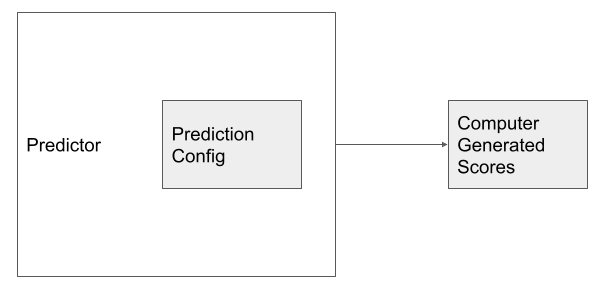
\includegraphics[width=0.3\textwidth]{pngs/predictor-1111.png}
%   \end{center}
%   \caption{The Predictor}\label{Fig:Data1}
%   \end{wrapfigure}

\section{The Predictor}

The Predictor is responsible for producing computer-generated scores. As described in the following figure, it takes a prediction configuration as input and produces scores based on this configuration.

\begin{figure}[h]
  \begin{minipage}{0.48\textwidth}
     \centering
     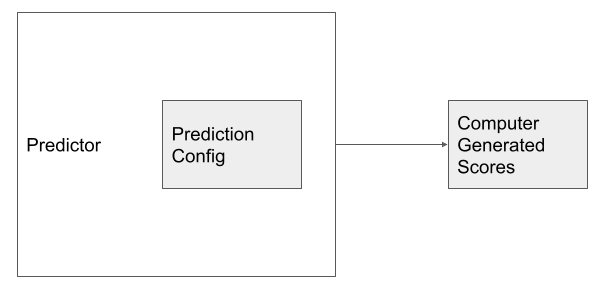
\includegraphics[width=.7\linewidth]{pngs/predictor-1111.png}
     \caption{The Predictor}\label{Fig:Data1}
  \end{minipage}\hfill
  \begin{minipage}{0.48\textwidth}
     \centering
     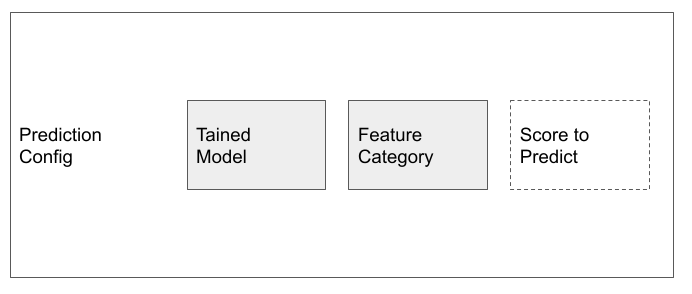
\includegraphics[width=.7\linewidth]{pngs/prediction-config.png}
     \caption{Prediction Configuration}\label{Fig:Data2}
  \end{minipage}
\end{figure}

% \begin{wrapfigure}{r}{0.4\textwidth}
%   \begin{center}
%     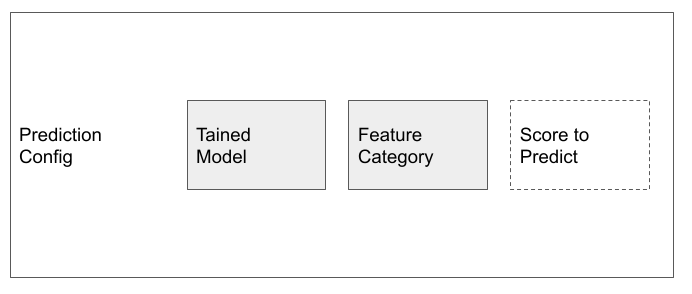
\includegraphics[width=0.3\textwidth]{pngs/prediction-config.png}
%   \end{center}
%   \caption{The Predictor}\label{Fig:Data1}
%   \end{wrapfigure}

\subsection{Prediction Configuration}

A Prediction Configuration, as seen below, is composed of a trained model, a feature category, and the target score to predict from the feature category. A trained model is a model which has an enhanced understanding of a relationship between an input and an output for a specific problem by being given examples of this problem from a specific dataset.  

% \begin{figure}[h]
%      \centering
%      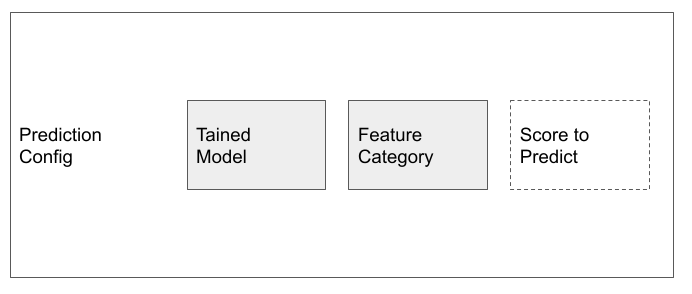
\includegraphics[width=.4\linewidth]{pngs/prediction-config.png}
%      \caption{AES as a Product}\label{Fig:Data1}
% \end{figure}

\subsection{The Prediction Configuration Generator}
The Prediction Configuration Generator (PCG)  is responsible for producing multiple prediction configuration objects. It can also be used to produce a single prediction configuration object, which may be useful after the evaluation stage of this project. 

For the experimental stage of this project, it was advantageous to produce prediction configuration permutations because it allowed us to explore the a variety of  Prediction Configurations. 

\begin{figure}[h]
   \begin{minipage}{0.48\textwidth}
     \centering
     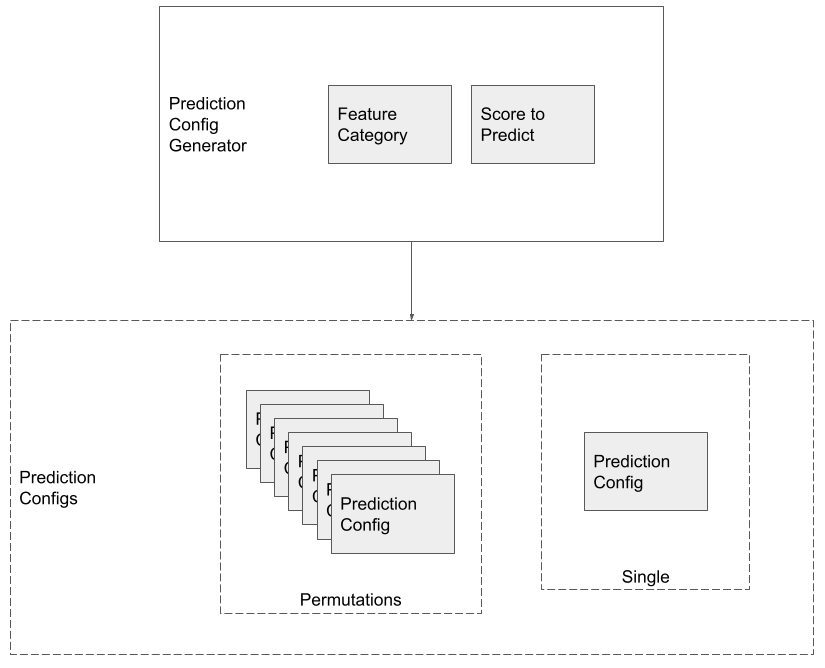
\includegraphics[width=.7\linewidth]{pngs/pcg-permutations.png}
     \caption{PCG: Permutator}\label{Fig:Data1}
   \end{minipage}\hfill
   \begin{minipage}{0.48\textwidth}
     \centering
     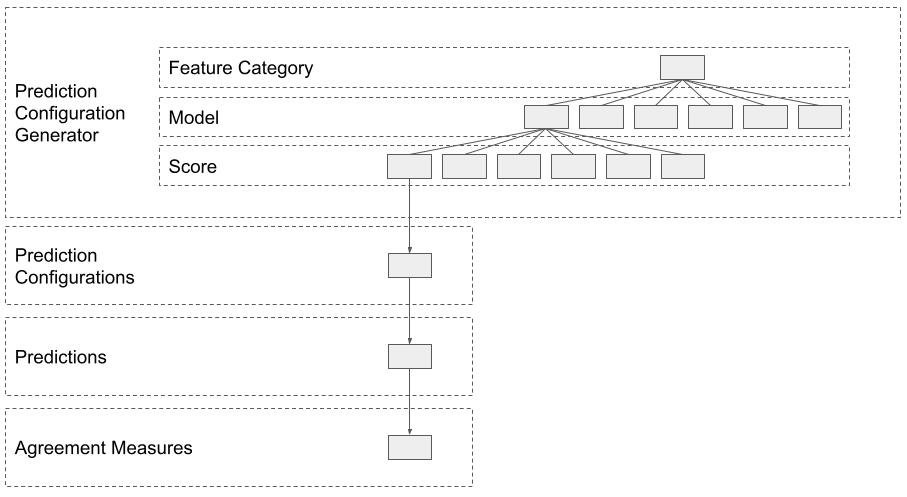
\includegraphics[width=.7\linewidth]{pngs/pcg-tree.png}
     \caption{PCG: Pipeline}\label{Fig:Data2}
   \end{minipage}
\end{figure}
\chapter{Implementation}\label{C:imp} 

% \begin{wrapfigure}{r}{0.3\textwidth}
%  \begin{center}
%   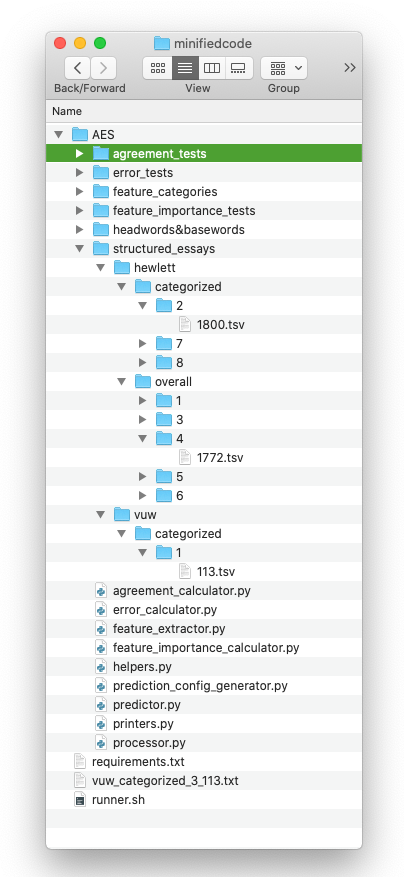
\includegraphics[width=0.25\textwidth]{pngs/struct.png}
%  \end{center}
%  \caption{Project Structure}
% \end{wrapfigure} 


\section{Development}

Initial programs were made using google-colab. This platform was beneficial in the exploration stage for programmatically investigating Natural Language Processing and Machine Learning. Following this, all implementation was done with Python in Visual Studio Code. Several libraries have been incorporated, such as Natural Language Toolkit, Language Check, Text Stat, Pandas, Matlab, Sklearn. Executions were orchestrated using Bash. Amazon's Elastic Cloud Compute (EC2) service was also used for executions. Amazon Elastic Compute Cloud is a part of Amazon.com's cloud-computing platform, Amazon Web Services, which allows users to rent virtual computers to run their computer applications.

\subsection{Structure}

The project's root is the "AES" folder, the requirements.txt, and the "runner.sh" which is the batch job orchestrator bash script. Also, all execution log files will appear at this level of the project. My reason for only having these files at this level is that the project is more runnable than a codebase. So all the things you need to execute any component can be done from here, and all log files will appear here without the clutter or mechanics of the python files that do the automatic scoring getting in the way.

Inside the AES folder is where all of the python code files, data, and artifacts live. The folders at this level are split into categories based on the artifacts that the project produces or consumes, such as; agreement tests, feature categories, headwords, and baseboards. Also, at this level are all of the python files. Again, this is pure to accommodate working with multiple files in Python. Splitting up the code as much as possible was a priority of mine as I wanted to keep the code abseils as manual as possible so that each opponent was easy to understand and there develop and debug. Although this does mean that there are several main files all at one place in eh director, this was worth it as I wanted to avoid creating a monolith. Again this was for my benefit as well as the future students of this project. Additionally, having well-defined separated responsibilities allows for a more straightforward explanation of the system to non-technical stakeholders. The location or folder structure of most artifacts, can be seen in the figure. I made this early design choice to standardise the general structure for any given dataset, of any version, being run against any component. This was a benefit as there is a lot of cross-pollination of the component ts. As they all produce and consume different artifices for each other. So having some unified rules around this was helpful. This is primarily due to the nature of my modularised system, where each component is frequently importing and exporting things.

% \begin{wrapfigure}{r}{0.5\textwidth}
%  \begin{center}
%   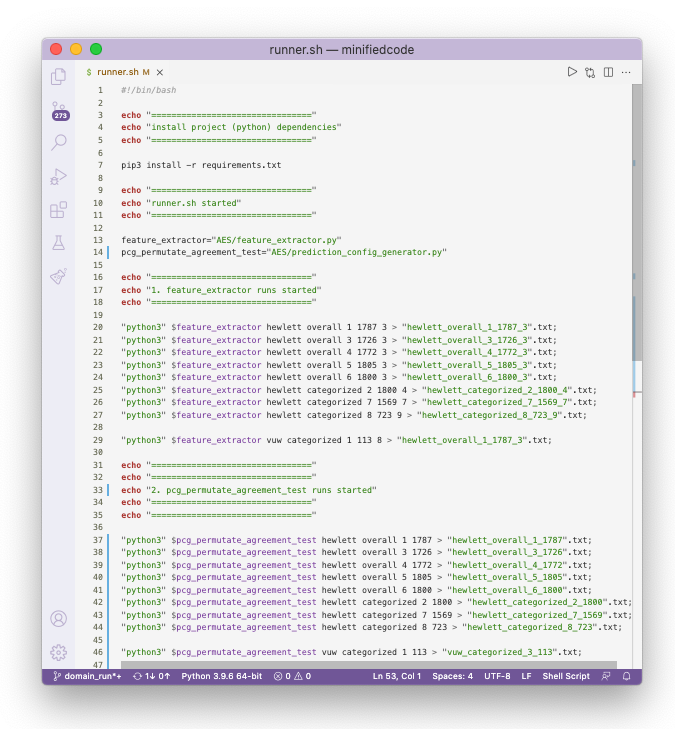
\includegraphics[width=0.55\textwidth]{pngs/runner.png}
%  \end{center}
%  \caption{Batch Job: Multiple Executions}
% \end{wrapfigure}

\subsection{Executions}
An execution can be thought of as running a component against a dataset. For example, common execution goals include running The Feature Extractor against the VUW EPP data to produce Feature Categories or running The PCG, The Predictor, and The Agreement Calculator against the Hewlett data to produce Agreement Measures. Often multiple executions are grouped and commenced with a single command, just like how a batch job might be done. A batch job can be considered a predefined group of processing actions with little or no interaction between the user and the system. In our case, this was often to run multiple datasets through the feature extractor, predictor, and agreement calculator. 

\subsection{Workflow}
The workflow for conducting an execution is described in the following diagram.

% \begin{figure}[h]
%   \centering
%   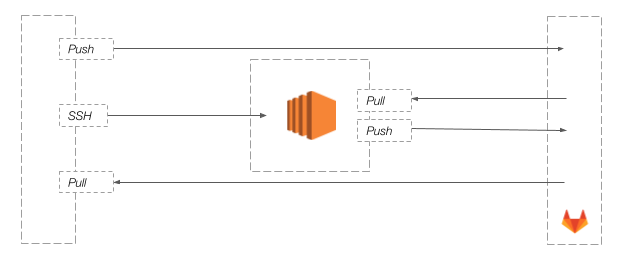
\includegraphics[width=.6\linewidth]{pngs/workflow-updated.png}
%   \caption{Workflow}
%   \label{Fig:Data1}
% \end{figure}

\paragraph{Push}
This step is required to provide the EC2 instance with the relevant resources that it may require for a proposed execution. These resources are committed and pushed from the local machine and then are retrieved or pulled from git before an execution. For example, if the proposed execution is to generate features for a new dataset, this would require committing and pushing the respective dataset's TSV file, provided it is in the correct location.

\paragraph{SSH} Once connected to the cloud instance. You can first pull from the remote to receive the newest version of the project on the instance. Following this, you can execute the runner script, which will execute predefined executions. After the bash script has been completed, you can then commit the newly created artifacts and push them to the remote to update them with the newly produced artifacts. While the bash script or runner is executing, you can observe the status of each job by viewing the associated log file. 

This was made possible by incorporating extensive logging for all types of execution. The motivation and gains of this are discussed in the following sections.

As many components interact, it was beneficial to have some form of sanity checking to help mitigate elementary mistakes or impossibilities that might be unclear when programming or are based on invalid assumptions. In addition, having this level of visibility helped to ensure the system was operating as I expected. This was especially helpful when ensuring intended permutations were being made, which datasets were being used, as developing and validating this process could get quite overwhelming otherwise.

Having these extensive logs also provided more information when troubleshooting or investigating bugs by providing more information. As well as this, for most systems of its maturity, the time to implement some form of incremental run-state backup system is not worth it. In most cases, for systems of this maturity, if the system is running a job and it encounters an error, the system will crash entirely, and its current task's progress will be lost. And unfortunately, until that problem is resolved, the same task will continue to fail until it is directly attended to.

Additionally, I chose to export this log data to a file as, over time, the amount of information I was outputting exceeded the console's memory limit. As well as this, it was tough to retrieve log statements when running in the cloud after exiting an ssh session for a process executed. However, it also meant that I could quickly and conveniently review a job's status post-run.

\paragraph{Pull} Once all executions have been completed or when you reconnect to the server, you can commit and push all new artifacts to the remote. Then you can exit the SSH session, and from your local machine, pull from the remote to receive all the newly produced artifacts.

\section{The Feature Extractor}

The Feature extractor can be broken down into the following main stages.

\paragraph{1. Initialise } In the Initialisation stage, one of the first things the AES will do is load any pre-existing resources that it may require, such as the headwords list, stop words list, and POS trigrams. Also, in this step, the system will initialize any necessary data structures, such as the lists for each feature category.

\paragraph{2. Import} In the import stage, the system will read and translate the relevant essay TSV into a two-dimensional array. The location of the relevant structured essay, as mentioned previously, will be derived from the run parameters.

\paragraph{3.} Then, for every essay, it will:

\paragraph{3.1. Process Identifiers} Here, the feature extractor will process the essays identifiers to all feature categories.

% \begin{wrapfigure}{l}{0.6\textwidth}
%  \begin{center}
%   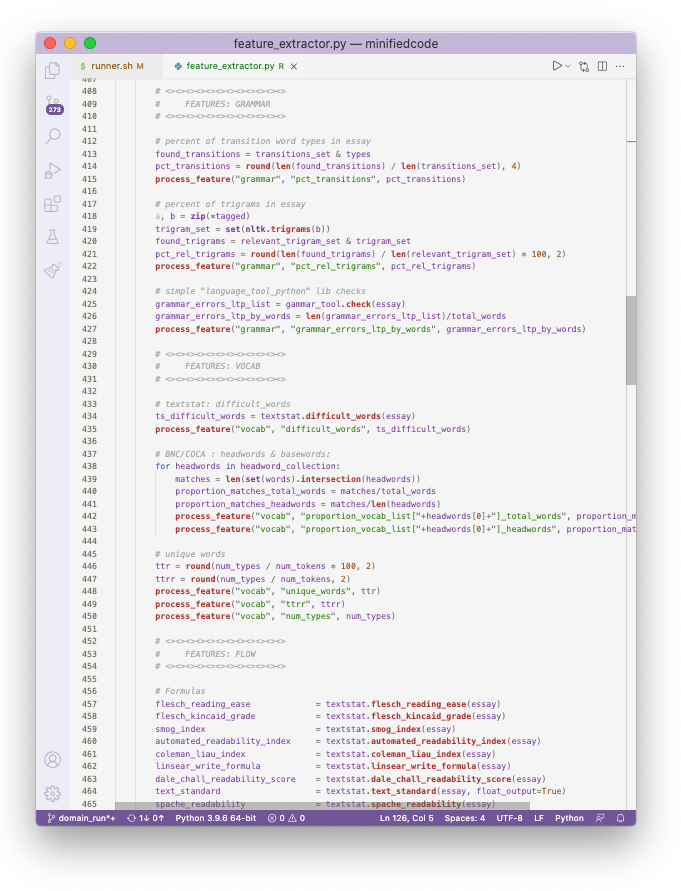
\includegraphics[width=0.55\textwidth]{pngs/feature-extract-code.png}
%  \end{center}
%  \caption{The Feature Extractor}
% \end{wrapfigure}

\paragraph{3.2. Process The Features} Processing a feature is done by performing a predefined calculation and then inputting the result of that calculation into the "processing" method along with a category. This method will then add the value or result of the feature to a list for the specific category and the overall category. This was done simply as a naive approach to categorising. Going forward, this should be updated. 

\paragraph{4. Export Feature Categories} Lastly, the Feature Extractor will translate the categorised data structures into separate TSV fikes. In order to produce feature categories containing all essays with only the feature values specific to themselves.

\subsection{Feature Importance Tests}

The future tests work by comparing the overall future category, which contains all features, to every categorical score using many helper methods from sklearn similar to the prediction component. 

% \begin{wrapfigure}{r}{0.5\textwidth}
%  \begin{center}
%   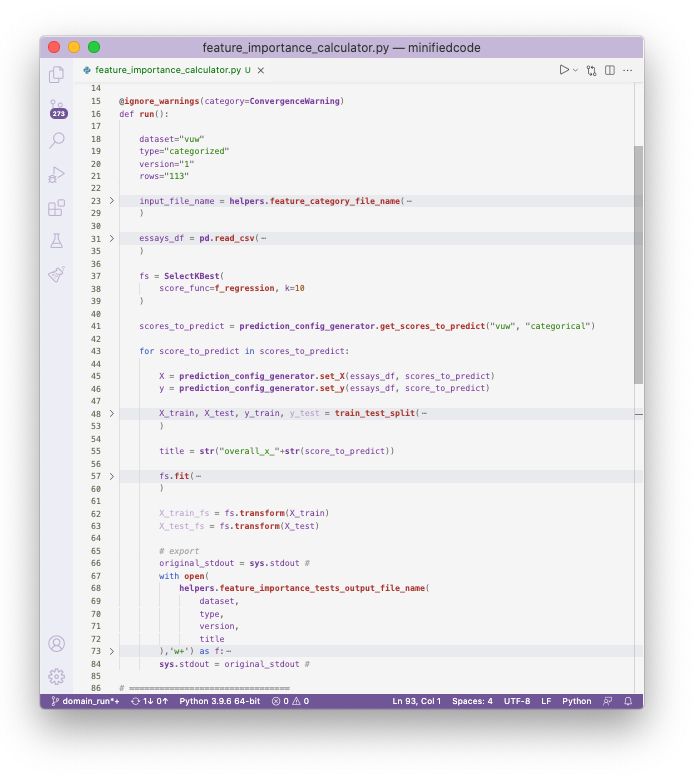
\includegraphics[width=0.48\textwidth]{pngs/feature-importance-code.png}
%  \end{center}
%  \caption{Feature Importance Tests}
% \end{wrapfigure}

\section{The Predictor}

From a programmatic perspective, the prediction component is relatively simple as it can be done in one line of code using the sklearn library. Therefore, in the final solution, this component will use the most optimal pre-trained model, for a category, from an imported ".pkl" file. However, for the duration of this project, these models only needed to persist at run time for a single execution. Therefore they did not need to be exported. 

% \begin{wrapfigure}{r}{0.5\textwidth}
%  \begin{center}
%   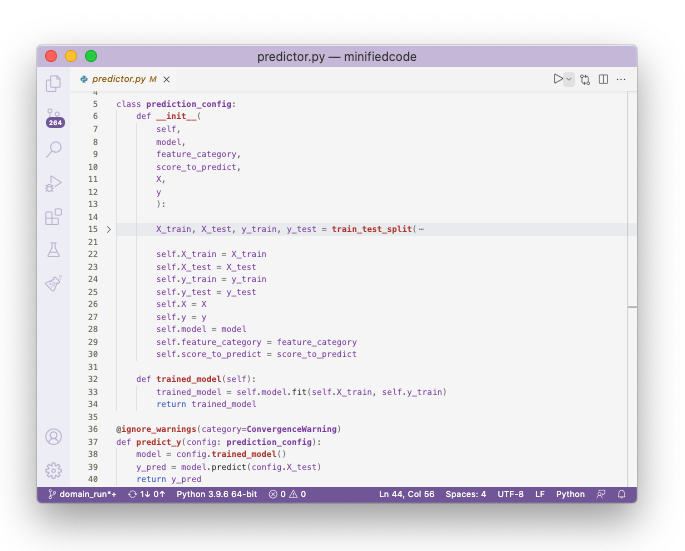
\includegraphics[width=0.48\textwidth]{pngs/predictor-code.png}
%  \end{center}
%  \caption{The Predictor}
% \end{wrapfigure}

\subsection{The Prediction Configuration Generator}

The Prediction Configuration Generator has two main methods. Permeate, and Run. They use the Prediction Configuration class, which stores a model, feature category, score to predict, and other fields. 
Having this simple class is super helpful for retaining an intended test's information.

The Permutate method mainly consists of a triple nested loop that loops through predefined models, feature categories, and scores to predict. The list of models remains the same for all execution types or configurations—however, the feature categories and scores to predict can vary depending on the execution params. For example, the scores to predict list for an "overall" run type only consist of the overall score. Each inner iteration will train a model, produce predictions, and compare them to the human-produce scores to produce agreement measures. One thing to note in this method is the outlier function. 

% \begin{figure}[h]
%   \begin{minipage}{0.48\textwidth}
%   \centering
%   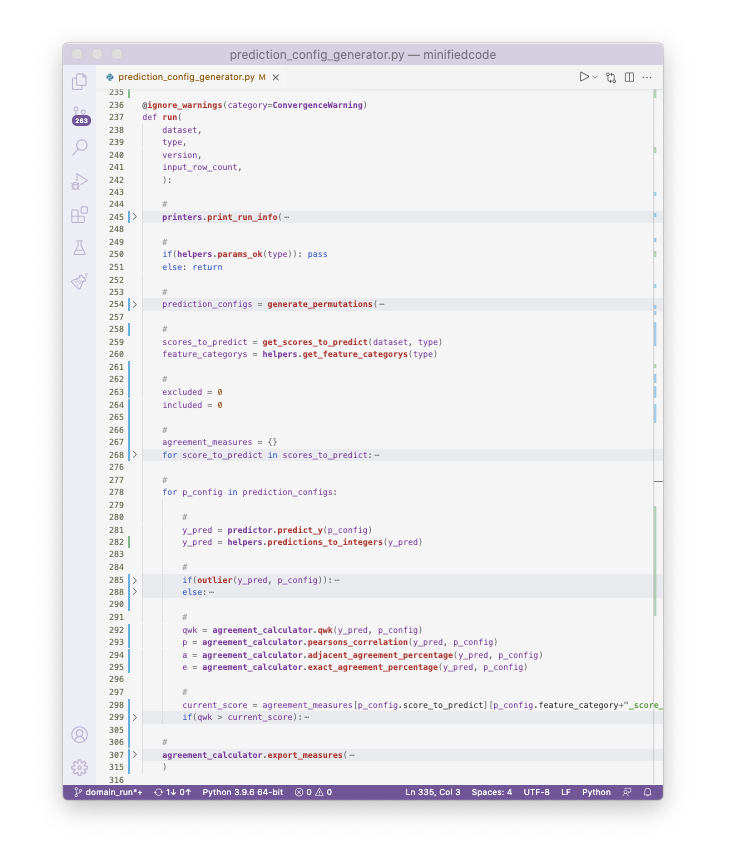
\includegraphics[width=.7\linewidth]{pngs/pcg.png}
%   \caption{Interpolation for Data 1}\label{Fig:Data1}
%   \end{minipage}\hfill
%   \begin{minipage}{0.48\textwidth}
%   \centering
%   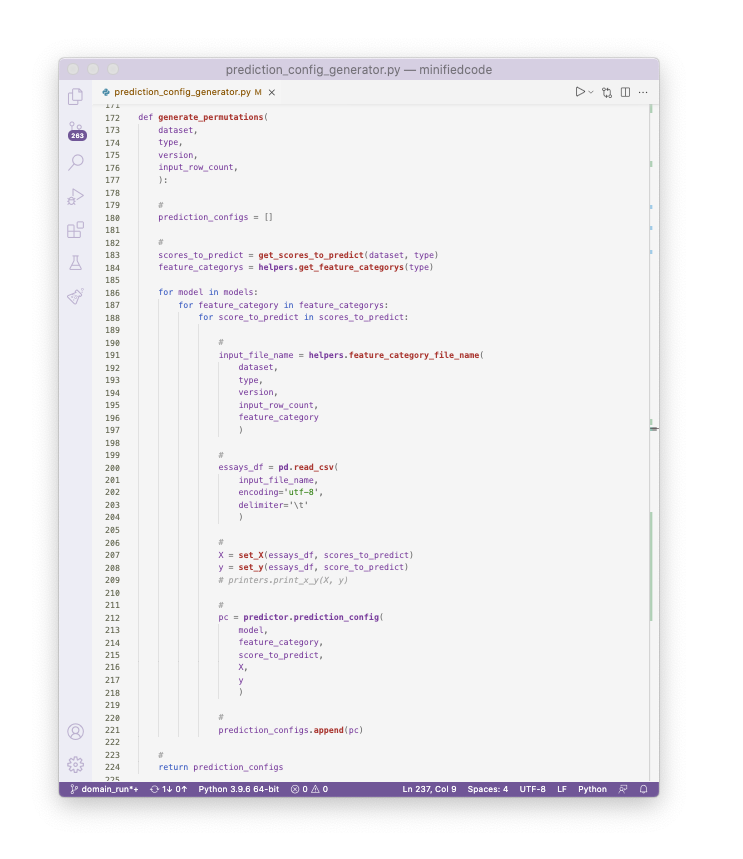
\includegraphics[width=.7\linewidth]{pngs/permutations.png}
%   \caption{Interpolation for Data 2}\label{Fig:Data2}
%   \end{minipage}
% \end{figure}

The motivation behind this was to avoid processing any tremendous prediction values generated by the computer. Not only did this take a very long time, but it also meant that Prediction Configuration was very, wildly inaccurate anyway. So it did not need to be consumed by the agreement calculator and component to the current best QWK because it would not be a suitable candidate for having the best QWK. 

The way these unusually high values are moderated is simply by calculating the mean of the prediction values list and comparing this to the mean of the actual human-generated scores list. If the mean is too big, the triple nested loop will end that iteration and start the logical next iteration.

To validate this, to make sure that I was not removing valuable test results. I implemented an "excluded "count and divided this by the size of the precision values list to get the percentage of Prediction Configurations being ignored. I have just left this debugging code in the system, and for all run's observed, the ignored configurations are a relatively small proportion.

\subsection{The Agreement Calculator}

The Agreement Calculator calculates the following measures: Quadratic Weighted Kappa, Pearson correlation coefficient, Adjacent Agreement Percentage, Exact Agreement Percentage. The logic and maths of the first two are mainly outsourced to sklean. The following two are both created manually. Most of these metrics do some mathematical operations on the human given scores and the computer-generated scores. 

% \begin{wrapfigure}{r}{0.5\textwidth}
%  \begin{center}
%   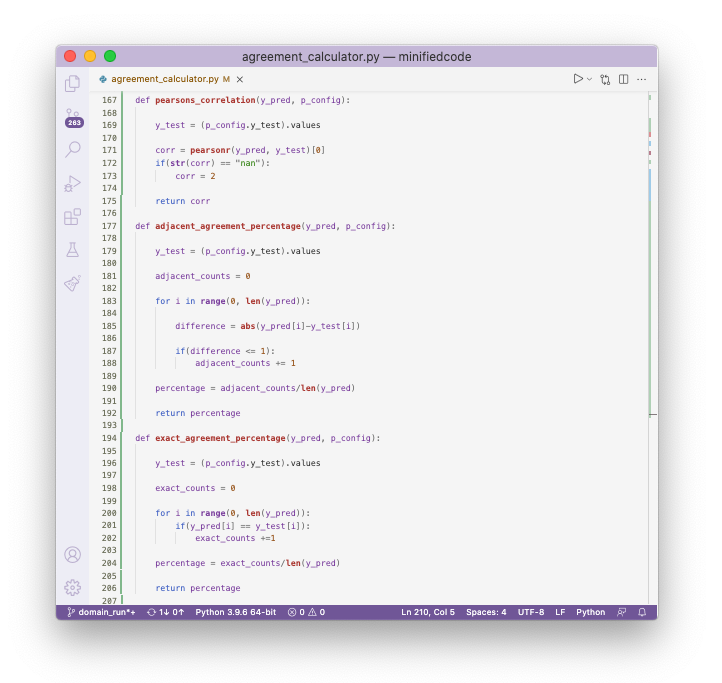
\includegraphics[width=0.48\textwidth]{pngs/agreement-calc.png}
%  \end{center}
%  \caption{The Agreement Measures}
% \end{wrapfigure}

In the case of the adjacent-agreement measure, this is calculated by comparing these two values, calculating the absolute difference between them, checking if the difference is one (or less), and if so, incrementing the adjacent count variable by 1. This is done until all pairs of values are checked. Then, following this, a percentage is calculated by dividing the adjacent counts by the total pairs. In the case of the exact agreements, the producer is very similar. However, we check whether both values are the same instead of calculating a difference between the computer and human-generated scores. If they are, a counter is incremented, and a percentage out of all predictions is calculated from this, like the other measure.

\chapter{Evaluation}\label{C:eval}

\section{The Feature Extractor}
Within The Feature Extractor, simply identifying a feature is a major breakthrough. However, this is a time consuming and complex process. Beyond this, the next most valuable task that can be is understanding if a feature is in the correct Feature Category. However, due to the nature of feature engineering, as it solely relies on domain knowledge, there is likely always room for further optimisation or refinement, beyond the initial discovery or identification of them. As a result, it is worthwhile to investigate to what extent a feature is actually aiding the predictive model to verify our assumptions of the domain and potentially optimise our system. 

\paragraph{Feature Importance Tests}
Feature Importance Tests can be useful for this. Feature Importance Tests refer to techniques that assign a score to input features based on how useful they are at predicting a target variable [x]. These give us an indication into whether or not our features are helping the predictor to synthesize a relationship between themselves and the score. 

The results can then be used to delete the features with the lowest scores or keep the features with the highest scores. This can simplify the problem that is being modeled, speed up the modeling process, and potentially, improve the performance of the model [x]. 

\paragraph{F-Value}
The values or scores of each feature are generated through an F-Test. The F-Test is a form of hypothesis testing. Where a model is created with just a constant and another model is created with a constant and a feature. Then the least squared errors in both the models are compared to checks if the difference in errors between each model is significant or introduced by chance [x].

Below are the features for each category that have the highest importance.
- I will compare the actual highest to the features that are currently being used.
- 

\subsubsection{Vocab}

Here we can see that 13 of the top 38 features are currently being used to predicting the Vocab score. This is $34\%$ of this range. However, 8 of the top 19 are being used to predict the Vocab score. Which is an improvement, at $50\%$. 

This is one of the higher proportions of strong features being used. However, the  vocab category has the most amount of features, excluding the overall category, due to it consisting of the headwords feature type. As the way this group of features is calculated is by producing a feature for each band of the headwords. Because of this, this would lead me to believe why there are a lot scores in the first two thirds of the tables.

% ==========================================
% Please add the following required packages to your document preamble:
% \usepackage{booktabs}
% \usepackage{graphicx}
% \usepackage[table,xcdraw]{xcolor}
% If you use beamer only pass "xcolor=table" option, i.e. \documentclass[xcolor=table]{beamer}
\begin{table}[h]
\centering
\resizebox{\textwidth}{!}{%
\begin{tabular}{@{}llllllll@{}}
\toprule
Feature &
  Score &
  &
  Feature &
  Score &
  &
  Feature &
  Score \\ \midrule
\cellcolor[HTML]{EFEFEF}\textbf{proportion\_vocab\_list{[}abandon{]}\_headwords} &
  \cellcolor[HTML]{EFEFEF}\textbf{22.05833729} &
  &
  nfunction\_tokens &
  5.704050657 &
  &
  \cellcolor[HTML]{EFEFEF}\textbf{proportion\_vocab\_list{[}abomasum{]}\_total\_words} &
  \cellcolor[HTML]{EFEFEF}\textbf{3.095114627} \\
\cellcolor[HTML]{EFEFEF}\textbf{proportion\_vocab\_list{[}accent{]}\_headwords} &
  \cellcolor[HTML]{EFEFEF}\textbf{16.40796885} &
  &
  ncontent\_types &
  5.219737871 &
  &
  \cellcolor[HTML]{EFEFEF}\textbf{proportion\_vocab\_list{[}abomasum{]}\_headwords} &
  \cellcolor[HTML]{EFEFEF}\textbf{3.095114627} \\
polysyllabcount &
  15.71130959 &
  &
  n\_trigram\_lemma\_types &
  5.118016095 &
  &
  \cellcolor[HTML]{EFEFEF}\textbf{total\_sentences} &
  \cellcolor[HTML]{EFEFEF}\textbf{3.078611375} \\
\cellcolor[HTML]{EFEFEF}\textbf{difficult\_words} &
  \cellcolor[HTML]{EFEFEF}\textbf{12.18352548} &
  &
  \cellcolor[HTML]{EFEFEF}\textbf{num\_types} &
  \cellcolor[HTML]{EFEFEF}\textbf{5.118016095} &
  &
  ncontent\_tokens &
  3.07783032 \\
determiners\_total &
  11.54240886 &
  &
  nlemma\_types &
  5.118016095 &
  &
  ts\_avg\_len\_sent &
  3.002896576 \\
smog\_index &
  9.174520901 &
  &
  n\_bigram\_lemma\_types &
  5.118016095 &
  &
  automated\_readability\_index &
  2.779641652 \\
determiners\_per\_words &
  8.446785067 &
  &
  crawford &
  4.81807535 &
  &
  monosyllabcount &
  2.616700091 \\
text\_standard &
  7.983828856 &
  &
  lexicon\_count &
  4.468261165 &
  &
  conjunctions\_total &
  2.568940715 \\
syllable\_count &
  7.092957374 &
  &
  \cellcolor[HTML]{EFEFEF}\textbf{proportion\_vocab\_list{[}aardvark{]}\_total\_words} &
  \cellcolor[HTML]{EFEFEF}\textbf{4.44829349} &
  &
  nfunction\_types &
  2.476570719 \\
\cellcolor[HTML]{EFEFEF}\textbf{proportion\_vocab\_list{[}abaft{]}\_headwords} &
  \cellcolor[HTML]{EFEFEF}\textbf{6.930334973} &
  &
  \cellcolor[HTML]{EFEFEF}\textbf{proportion\_vocab\_list{[}aardvark{]}\_headwords} &
  \cellcolor[HTML]{EFEFEF}\textbf{4.44829349} &
  &
  pct\_transitions &
  2.444242565 \\
\cellcolor[HTML]{EFEFEF}\textbf{proportion\_vocab\_list{[}abaft{]}\_total\_words} &
  \cellcolor[HTML]{EFEFEF}\textbf{6.895066765} &
  &
  nlemmas &
  4.300215352 &
  &
  spache\_readability &
  2.440962422 \\
\cellcolor[HTML]{EFEFEF}\textbf{proportion\_vocab\_list{[}abandon{]}\_total\_words} &
  \cellcolor[HTML]{EFEFEF}\textbf{6.703801959} &
  &
  n\_trigram\_lemmas &
  4.300215352 &
  &
  \cellcolor[HTML]{EFEFEF}\textbf{words\_div\_sentences} &
  \cellcolor[HTML]{EFEFEF}\textbf{2.37079476} \\
\cellcolor[HTML]{EFEFEF}\textbf{proportion\_vocab\_list{[}absentminded{]}\_total\_words} &
  \cellcolor[HTML]{EFEFEF}\textbf{6.424550614} &
  &
  n\_bigram\_lemmas &
  4.300215352 &
  &
  flesch\_kincaid\_grade &
  2.231981694 \\
\cellcolor[HTML]{EFEFEF}\textbf{proportion\_vocab\_list{[}accent{]}\_total\_words} &
  \cellcolor[HTML]{EFEFEF}\textbf{6.358088016} &
  &
  \cellcolor[HTML]{EFEFEF}\textbf{proportion\_vocab\_list{[}a{]}\_total\_words} &
  \cellcolor[HTML]{EFEFEF}\textbf{4.274963711} &
  &
  \cellcolor[HTML]{EFEFEF}\textbf{proportion\_vocab\_list{[}abashed{]}\_total\_words} &
  \cellcolor[HTML]{EFEFEF}\textbf{2.144350221} \\
function\_ttr &
  6.283303783 &
  &
  \cellcolor[HTML]{EFEFEF}\textbf{total\_words} &
  \cellcolor[HTML]{EFEFEF}\textbf{4.246082192} &
  &
  \cellcolor[HTML]{EFEFEF}\textbf{proportion\_vocab\_list{[}abashed{]}\_headwords} &
  \cellcolor[HTML]{EFEFEF}\textbf{2.144350221} \\
grammar\_errors\_ltp\_by\_words &
  5.873555877 &
  &
  pct\_rel\_trigrams &
  4.07939033 &
  &
  coleman\_liau\_index &
  1.978447928 \\
letter\_count &
  5.856224883 &
  &
  pronouns\_total &
  3.865049524 &
  &
  pronouns\_noun\_ratio &
  1.765296516 \\
reading\_time &
  5.742222651 &
  &
  ts\_avg\_syllab\_per\_word &
  3.349429602 &
  &
  pronouns\_density &
  1.74673426 \\
char\_count &
  5.742099891 &
  &
  sentence\_count &
  3.194236862 &
  &
  \cellcolor[HTML]{EFEFEF}\textbf{proportion\_vocab\_list{[}a{]}\_headwords} &
  \cellcolor[HTML]{EFEFEF}\textbf{1.739721638} \\ \bottomrule
\end{tabular}%
}
\caption{Vocab Feature Importance Tests}
\label{tab:e1}
\end{table}
% ==========================================

\subsubsection{Ideas}

Here we can see that 2 of the top 38 features are currently being used to predict the Vocab score. This is $5\%$ of this range, which is very low. Additionally, 1 of the top 19 are being used to predict the Vocab score. Which is also $5\%$.

The vocab category has the most amount of features, excluding the overall category, due to it consisting of the headwords feature type. As the way this group of features is calculated is by producing a feature for each band of the headwords. Because of this, this would lead me to believe why there are a lot scores in the first two thirds of the tables.

These results are potentially some of the most valuable. As this category was and the most neglected due to its complexity. The marking criteria definition for the high end scores of the Ideas category is "Development of ideas is deep and convincing." For this reason, the category only consisted of the "miscellaneous" features which were added to all feature categories. These include: total words total sentences and sentence density. 

% ==========================================
% Please add the following required packages to your document preamble:
% \usepackage{booktabs}
% \usepackage{graphicx}
% \usepackage[table,xcdraw]{xcolor}
% If you use beamer only pass "xcolor=table" option, i.e. \documentclass[xcolor=table]{beamer}
\begin{table}[h]
\centering
\resizebox{\textwidth}{!}{%
\begin{tabular}{@{}llllllll@{}}
\toprule
Feature &
  Score &
  &
  Feature &
  Score &
  &
  Feature &
  Score \\ \midrule
determiners\_total &
  23.98975321 &
  &
  monosyllabcount &
  17.06445867 &
  &
  pronouns\_density &
  2.86945213 \\
syllable\_count &
  22.65767743 &
  &
  polysyllabcount &
  16.01149404 &
  &
  content\_ttr &
  2.796727653 \\
letter\_count &
  21.76693064 &
  &
  proportion\_vocab\_list{[}a{]}\_headwords &
  15.05858081 &
  &
  ttr\_nouns &
  2.708399971 \\
reading\_time &
  21.50866321 &
  &
  nouns\_total &
  14.93762526 &
  &
  conjunctions\_unique &
  2.399994321 \\
char\_count &
  21.50722445 &
  &
  ncontent\_types &
  14.48729494 &
  &
  pronouns\_unique &
  2.399994321 \\
nfunction\_tokens &
  21.03021095 &
  &
  pct\_transitions &
  14.19203036 &
  &
  ts\_avg\_sent\_per\_word &
  2.38213524 \\
nfunction\_types &
  20.2273507 &
  &
  proportion\_vocab\_list{[}a{]}\_total\_words &
  12.68306971 &
  &
  proportion\_vocab\_list{[}abomasum{]}\_total\_words &
  2.296469714 \\
function\_ttr &
  20.22092973 &
  &
  pronouns\_total &
  11.80391532 &
  &
  proportion\_vocab\_list{[}abomasum{]}\_headwords &
  2.296469714 \\
lexicon\_count &
  20.04425343 &
  &
  difficult\_words &
  11.43922304 &
  &
  proportion\_vocab\_list{[}aal{]}\_total\_words &
  1.736032636 \\
nlemmas &
  19.87833192 &
  &
  conjunctions\_total &
  9.925480901 &
  &
  \cellcolor[HTML]{EFEFEF}\textbf{sent\_density} &
  \cellcolor[HTML]{EFEFEF}\textbf{1.494882434} \\
n\_bigram\_lemmas &
  19.87833192 &
  &
  proportion\_vocab\_list{[}accent{]}\_headwords &
  9.86627013 &
  &
  proportion\_vocab\_list{[}a1{]}\_total\_words &
  1.231983429 \\
n\_trigram\_lemmas &
  19.87833192 &
  &
  \cellcolor[HTML]{EFEFEF}\textbf{total\_sentences} &
  \cellcolor[HTML]{EFEFEF}\textbf{9.683989634} &
  &
  pronouns\_noun\_ratio &
  1.22992392 \\
\cellcolor[HTML]{EFEFEF}\textbf{total\_words} &
  \cellcolor[HTML]{EFEFEF}\textbf{19.58377946} &
  &
  sentence\_count &
  9.665452001 &
  &
  text\_standard &
  1.229178768 \\
pct\_rel\_trigrams &
  18.84225246 &
  &
  ttrr &
  9.10015428 &
  &
  linsear\_write\_formula &
  1.195434814 \\
ncontent\_tokens &
  17.70236467 &
  &
  unique\_words &
  9.080102356 &
  &
  proportion\_vocab\_list{[}absentminded{]}\_headwords &
  1.191540578 \\
n\_trigram\_lemma\_types &
  17.21977037 &
  &
  nouns\_unique &
  7.210491094 &
  &
  proportion\_vocab\_list{[}abalone{]}\_total\_words &
  1.10443711 \\
num\_types &
  17.21977037 &
  &
  proportion\_vocab\_list{[}abandon{]}\_headwords &
  4.724206672 &
  &
  proportion\_vocab\_list{[}abalone{]}\_headwords &
  1.10443711 \\
nlemma\_types &
  17.21977037 &
  &
  determiners\_per\_words &
  4.698053181 &
  &
  dale\_chall\_readability\_score &
  1.059783983 \\
n\_bigram\_lemma\_types &
  17.21977037 &
  &
  proportion\_vocab\_list{[}aal{]}\_headwords &
  4.37518797 &
  &
  proportion\_vocab\_list{[}abandon{]}\_total\_words &
  0.7944183939 \\ \bottomrule
\end{tabular}%
}
\caption{Ideas Feature Importance Tests}
\label{tab:e2}
\end{table}
% ==========================================

\subsubsection{Grammar}

Here we can see that 5 of the top 38 features are currently being used to predicting the Grammar score. This is $13\%$ of the most important features for this range. For the next range, we see similar results as 3 of the top 19 are being used to predict the Grammar score. Which is a slight at $15\%$.

This feature only consisted of three features although I was very confident in the grammar errors feature as I assumed this would be very strongly related. This assumption has (lucky) proven correct in the results as it is the strongest feature. Additionally, the remaining grammar-unique features from this category are within the top 19 features. 

However, despite the fact that the  current features for this category are important. There simply is just enough of them. 

% ==========================================
% Please add the following required packages to your document preamble:
% \usepackage{booktabs}
% \usepackage{graphicx}
% \usepackage[table,xcdraw]{xcolor}
% If you use beamer only pass "xcolor=table" option, i.e. \documentclass[xcolor=table]{beamer}
\begin{table}[h]
\centering
\resizebox{\textwidth}{!}{%
\begin{tabular}{@{}llllllll@{}}
\toprule
Feature &
  Score &
  &
  Feature &
  Score &
  &
  Feature &
  Score \\ \midrule
\cellcolor[HTML]{EFEFEF}\textbf{grammar\_errors\_ltp\_by\_words} &
  \cellcolor[HTML]{EFEFEF}\textbf{13.86887276} &
  &
  n\_trigram\_lemmas &
  8.428847883 &
  &
  proportion\_vocab\_list{[}abomasum{]}\_total\_words &
  3.447080979 \\
polysyllabcount &
  13.5453572 &
  &
  proportion\_vocab\_list{[}accent{]}\_headwords &
  8.335462779 &
  &
  proportion\_vocab\_list{[}abomasum{]}\_headwords &
  3.447080979 \\
determiners\_total &
  11.99318654 &
  &
  \cellcolor[HTML]{EFEFEF}\textbf{total\_words} &
  \cellcolor[HTML]{EFEFEF}\textbf{8.332141187} &
  &
  smog\_index &
  2.652814039 \\
syllable\_count &
  11.06434199 &
  &
  ncontent\_types &
  7.590394235 &
  &
  proportion\_vocab\_list{[}abnormal{]}\_total\_words &
  2.578601176 \\
letter\_count &
  9.777308962 &
  &
  ncontent\_tokens &
  7.000690642 &
  &
  proportion\_vocab\_list{[}aback{]}\_headwords &
  2.451993818 \\
nfunction\_tokens &
  9.676747576 &
  &
  proportion\_vocab\_list{[}a{]}\_headwords &
  6.970460707 &
  &
  proportion\_vocab\_list{[}aback{]}\_total\_words &
  2.412191877 \\
reading\_time &
  9.589911019 &
  &
  monosyllabcount &
  6.821351862 &
  &
  proportion\_vocab\_list{[}abaft{]}\_total\_words &
  2.159653449 \\
char\_count &
  9.587821097 &
  &
  proportion\_vocab\_list{[}abnormal{]}\_headwords &
  6.794462298 &
  &
  proportion\_vocab\_list{[}abaft{]}\_headwords &
  2.037732545 \\
difficult\_words &
  9.085364454 &
  &
  function\_ttr &
  5.868971179 &
  &
  nouns\_unique &
  2.03145763 \\
\cellcolor[HTML]{EFEFEF}\textbf{pct\_rel\_trigrams} &
  \cellcolor[HTML]{EFEFEF}\textbf{8.874333893} &
  &
  proportion\_vocab\_list{[}abandon{]}\_headwords &
  5.325501914 &
  &
  proportion\_vocab\_list{[}absentminded{]}\_total\_words &
  2.008426737 \\
nfunction\_types &
  8.78489224 &
  &
  \cellcolor[HTML]{EFEFEF}\textbf{total\_sentences} &
  \cellcolor[HTML]{EFEFEF}\textbf{4.777733853} &
  &
  proportion\_vocab\_list{[}abashed{]}\_total\_words &
  1.807824726 \\
\cellcolor[HTML]{EFEFEF}\textbf{pct\_transitions} &
  \cellcolor[HTML]{EFEFEF}\textbf{8.683182431} &
  &
  sentence\_count &
  4.665500367 &
  &
  proportion\_vocab\_list{[}abashed{]}\_headwords &
  1.807824726 \\
lexicon\_count &
  8.642680781 &
  &
  pronouns\_total &
  3.991921505 &
  &
  text\_standard &
  1.679480615 \\
n\_trigram\_lemma\_types &
  8.633375961 &
  &
  determiners\_per\_words &
  3.877961209 &
  &
  ttrr &
  1.666647575 \\
num\_types &
  8.633375961 &
  &
  conjunctions\_total &
  3.595950896 &
  &
  crawford &
  1.66445437 \\
nlemma\_types &
  8.633375961 &
  &
  proportion\_vocab\_list{[}a{]}\_total\_words &
  3.561214109 &
  &
  unique\_words &
  1.496118802 \\
n\_bigram\_lemma\_types &
  8.633375961 &
  &
  nouns\_total &
  3.448940441 &
  &
  linsear\_write\_formula &
  1.48898339 \\
nlemmas &
  8.428847883 &
  &
  proportion\_vocab\_list{[}abet{]}\_total\_words &
  3.447080979 &
  &
  proportion\_vocab\_list{[}a1{]}\_total\_words &
  1.389620477 \\
n\_bigram\_lemmas &
  8.428847883 &
  &
  proportion\_vocab\_list{[}abet{]}\_headwords &
  3.447080979 &
  &
  ts\_avg\_sent\_per\_word &
  0.7677552826 \\ \bottomrule
\end{tabular}%
}
\caption{Grammar Feature Importance Tests}
\label{tab:e3}
\end{table}
% ==========================================

\subsubsection{Flow}

Here we can see that 10 of the top 38 features are currently being used to predict the Flow score. This is $26\%$ of the most important features for this range. For the next range, we see the exact same results as 5 of the top 19 are being used to predict the Grammar score. Which is $26\%$ of this range.

This feature consists of a huge amount of imported libraries that calculate readability measures for the text. For this reason, I find it quite surprising that there is not a greater percentage for these measures with these ranges. Five of the twelve readability measures are evident in the top 38 features.

% ==========================================
% Please add the following required packages to your document preamble:
% \usepackage{booktabs}
% \usepackage{graphicx}
% \usepackage[table,xcdraw]{xcolor}
% If you use beamer only pass "xcolor=table" option, i.e. \documentclass[xcolor=table]{beamer}
\begin{table}[h]
\centering
\resizebox{\textwidth}{!}{%
\begin{tabular}{@{}llllllll@{}}
\toprule
Feature &
  Score &
  &
  Feature &
  Score &
  &
  Feature &
  Score \\ \midrule
grammar\_errors\_ltp\_by\_words &
  10.52322172 &
  &
  \cellcolor[HTML]{EFEFEF}\textbf{reading\_time} &
  \cellcolor[HTML]{EFEFEF}\textbf{3.446741393} &
  &
  \cellcolor[HTML]{EFEFEF}\textbf{linsear\_write\_formula} &
  \cellcolor[HTML]{EFEFEF}\textbf{2.179626868} \\
proportion\_vocab\_list{[}accent{]}\_headwords &
  8.616507797 &
  &
  \cellcolor[HTML]{EFEFEF}\textbf{char\_count} &
  \cellcolor[HTML]{EFEFEF}\textbf{3.445241765} &
  &
  proportion\_vocab\_list{[}a{]}\_total\_words &
  1.970600376 \\
proportion\_vocab\_list{[}abaft{]}\_headwords &
  7.174452719 &
  &
  nfunction\_types &
  3.25497433 &
  &
  proportion\_vocab\_list{[}aback{]}\_total\_words &
  1.786283529 \\
proportion\_vocab\_list{[}abaft{]}\_total\_words &
  7.137848797 &
  &
  \cellcolor[HTML]{EFEFEF}\textbf{crawford} &
  \cellcolor[HTML]{EFEFEF}\textbf{3.153343606} &
  &
  \cellcolor[HTML]{EFEFEF}\textbf{monosyllabcount} &
  \cellcolor[HTML]{EFEFEF}\textbf{1.743636837} \\
pct\_transitions &
  5.952052458 &
  &
  proportion\_vocab\_list{[}abet{]}\_total\_words &
  2.785493827 &
  &
  proportion\_vocab\_list{[}aal{]}\_total\_words &
  1.605845889 \\
\cellcolor[HTML]{EFEFEF}\textbf{polysyllabcount} &
  \cellcolor[HTML]{EFEFEF}\textbf{5.908466276} &
  &
  proportion\_vocab\_list{[}abet{]}\_headwords &
  2.785493827 &
  &
  proportion\_vocab\_list{[}abrasion{]}\_headwords &
  1.539322698 \\
difficult\_words &
  5.813492969 &
  &
  \cellcolor[HTML]{EFEFEF}\textbf{lexicon\_count} &
  \cellcolor[HTML]{EFEFEF}\textbf{2.775661365} &
  &
  pronouns\_total &
  1.371066736 \\
\cellcolor[HTML]{EFEFEF}\textbf{text\_standard} &
  \cellcolor[HTML]{EFEFEF}\textbf{4.888289364} &
  &
  proportion\_vocab\_list{[}a{]}\_headwords &
  2.771527007 &
  &
  \cellcolor[HTML]{EFEFEF}\textbf{coleman\_liau\_index} &
  \cellcolor[HTML]{EFEFEF}\textbf{1.332429938} \\
proportion\_vocab\_list{[}abandon{]}\_headwords &
  4.575020547 &
  &
  \cellcolor[HTML]{EFEFEF}\textbf{total\_words} &
  \cellcolor[HTML]{EFEFEF}\textbf{2.733166972} &
  &
  proportion\_vocab\_list{[}aback{]}\_headwords &
  1.320345559 \\
n\_trigram\_lemma\_types &
  4.263709123 &
  &
  nlemmas &
  2.66E+00 &
  &
  \cellcolor[HTML]{EFEFEF}\textbf{total\_sentences} &
  \cellcolor[HTML]{EFEFEF}\textbf{1.119213959} \\
num\_types &
  4.263709123 &
  &
  n\_bigram\_lemmas &
  2.661185087 &
  &
  \cellcolor[HTML]{EFEFEF}\textbf{sentence\_count} &
  \cellcolor[HTML]{EFEFEF}\textbf{1.118883069} \\
nlemma\_types &
  4.263709123 &
  &
  n\_trigram\_lemmas &
  2.661185087 &
  &
  proportion\_vocab\_list{[}aardvark{]}\_total\_words &
  0.9790015297 \\
n\_bigram\_lemma\_types &
  4.263709123 &
  &
  ncontent\_tokens &
  2.62501352 &
  &
  proportion\_vocab\_list{[}aardvark{]}\_headwords &
  0.9790015297 \\
\cellcolor[HTML]{EFEFEF}\textbf{syllable\_count} &
  \cellcolor[HTML]{EFEFEF}\textbf{4.156071732} &
  &
  determiners\_total &
  2.558186665 &
  &
  sent\_density &
  0.9545624739 \\
pct\_rel\_trigrams &
  4.011612142 &
  &
  nfunction\_tokens &
  2.530773085 &
  &
  proportion\_vocab\_list{[}abate{]}\_total\_words &
  0.9144704138 \\
ncontent\_types &
  4.011139066 &
  &
  proportion\_vocab\_list{[}absentminded{]}\_total\_words &
  2.46882231 &
  &
  proportion\_vocab\_list{[}abnormal{]}\_headwords &
  0.90326088 \\
function\_ttr &
  3.796428186 &
  &
  proportion\_vocab\_list{[}accent{]}\_total\_words &
  2.23868793 &
  &
  proportion\_vocab\_list{[}abate{]}\_headwords &
  0.8364237459 \\
\cellcolor[HTML]{EFEFEF}\textbf{letter\_count} &
  \cellcolor[HTML]{EFEFEF}\textbf{3.528072315} &
  &
  proportion\_vocab\_list{[}abashed{]}\_total\_words &
  2.215948697 &
  &
  nouns\_total &
  0.8331892199 \\
\cellcolor[HTML]{EFEFEF}\textbf{smog\_index} &
  \cellcolor[HTML]{EFEFEF}\textbf{3.499672392} &
  &
  proportion\_vocab\_list{[}abashed{]}\_headwords &
  2.215948697 &
  &
  conjunctions\_unique &
  0.8321611094 \\ \bottomrule
\end{tabular}%
}
\caption{Flow Feature Importance Tests}
\end{table}
% ==========================================

\subsubsection{Coherence}

Here we can see that 16 of the top 38 features are currently being used to predict the Coherence score. This is $42\%$ of this range, which is the highest percentage of all of categories for this range (excluding the overall category). Additionally, 8 of the top 19 are being used to predict the Coherence score. Which is the again, the highest percentage of all of the categories for this range (excluding the overall category), at $50\%$. 

This score has the features with the highest percentage of important features in both bands. However, it does have the second largest amount of features, excluding the overall category. As the way this group of features is calculated is by producing a feature for each band of the headwords. Because of this, this would lead me to believe why there are a lot scores in the first two thirds of the tables.

% ==========================================
% Please add the following required packages to your document preamble:
% \usepackage{booktabs}
% \usepackage{graphicx}
% \usepackage[table,xcdraw]{xcolor}
% If you use beamer only pass "xcolor=table" option, i.e. \documentclass[xcolor=table]{beamer}
\begin{table}[h]
\centering
\resizebox{\textwidth}{!}{%
\begin{tabular}{@{}llllllll@{}}
\cmidrule(r){1-2} \cmidrule(lr){4-5} \cmidrule(l){7-8}
Feature &
  Score &
  &
  Feature &
  Score &
  &
  Feature &
  Score \\ \cmidrule(r){1-2} \cmidrule(lr){4-5} \cmidrule(l){7-8} 
pct\_transitions &
  20.68884211 &
  &
  \cellcolor[HTML]{EFEFEF}\textbf{pronouns\_total} &
  \cellcolor[HTML]{EFEFEF}\textbf{8.5764678} &
  &
  \cellcolor[HTML]{EFEFEF}{\color[HTML]{000000} \textbf{pronouns\_density}} &
  \cellcolor[HTML]{EFEFEF}{\color[HTML]{000000} \textbf{3.860901774}} \\
polysyllabcount &
  17.13412183 &
  &
  monosyllabcount &
  8.14921556 &
  &
  proportion\_vocab\_list{[}a1{]}\_total\_words &
  3.355255868 \\
pct\_rel\_trigrams &
  14.92687473 &
  &
  \cellcolor[HTML]{EFEFEF}\textbf{n\_trigram\_lemma\_types} &
  \cellcolor[HTML]{EFEFEF}\textbf{7.57892787} &
  &
  crawford &
  3.083923886 \\
syllable\_count &
  13.17692848 &
  &
  num\_types &
  7.57892787 &
  &
  proportion\_vocab\_list{[}abnormal{]}\_headwords &
  3.059688495 \\
\cellcolor[HTML]{EFEFEF}\textbf{nfunction\_tokens} &
  \cellcolor[HTML]{EFEFEF}\textbf{11.94914458} &
  &
  \cellcolor[HTML]{EFEFEF}\textbf{nlemma\_types} &
  \cellcolor[HTML]{EFEFEF}\textbf{7.57892787} &
  &
  sentence\_count &
  2.858495234 \\
letter\_count &
  11.73462468 &
  &
  \cellcolor[HTML]{EFEFEF}\textbf{n\_bigram\_lemma\_types} &
  \cellcolor[HTML]{EFEFEF}\textbf{7.57892787} &
  &
  \cellcolor[HTML]{EFEFEF}\textbf{total\_sentences} &
  \cellcolor[HTML]{EFEFEF}\textbf{2.780063655} \\
proportion\_vocab\_list{[}abandon{]}\_headwords &
  11.47026469 &
  &
  \cellcolor[HTML]{EFEFEF}\textbf{ncontent\_tokens} &
  \cellcolor[HTML]{EFEFEF}\textbf{7.555855104} &
  &
  proportion\_vocab\_list{[}absentminded{]}\_total\_words &
  2.685789236 \\
reading\_time &
  11.40182309 &
  &
  proportion\_vocab\_list{[}a{]}\_total\_words &
  7.412367857 &
  &
  \cellcolor[HTML]{EFEFEF}\textbf{ttr\_nouns} &
  \cellcolor[HTML]{EFEFEF}\textbf{2.41010852} \\
char\_count &
  11.39842839 &
  &
  difficult\_words &
  6.882954381 &
  &
  ts\_avg\_sent\_per\_word &
  2.248255026 \\
\cellcolor[HTML]{EFEFEF}\textbf{function\_ttr} &
  \cellcolor[HTML]{EFEFEF}\textbf{10.84975839} &
  &
  proportion\_vocab\_list{[}aback{]}\_headwords &
  6.814253694 &
  &
  proportion\_vocab\_list{[}abet{]}\_total\_words &
  2.182106948 \\
grammar\_errors\_ltp\_by\_words &
  10.77253679 &
  &
  proportion\_vocab\_list{[}a{]}\_headwords &
  6.698095193 &
  &
  proportion\_vocab\_list{[}abet{]}\_headwords &
  2.182106948 \\
lexicon\_count &
  10.08744734 &
  &
  \cellcolor[HTML]{EFEFEF}\textbf{ncontent\_types} &
  \cellcolor[HTML]{EFEFEF}\textbf{6.48683046} &
  &
  proportion\_vocab\_list{[}abomasum{]}\_total\_words &
  2.182106948 \\
\cellcolor[HTML]{EFEFEF}\textbf{determiners\_total} &
  \cellcolor[HTML]{EFEFEF}\textbf{9.994962745} &
  &
  text\_standard &
  5.44173295 &
  &
  proportion\_vocab\_list{[}abomasum{]}\_headwords &
  2.182106948 \\
\cellcolor[HTML]{EFEFEF}\textbf{nlemmas} &
  \cellcolor[HTML]{EFEFEF}\textbf{9.723691954} &
  &
  proportion\_vocab\_list{[}accent{]}\_headwords &
  4.88851034 &
  &
  \cellcolor[HTML]{EFEFEF}\textbf{pronouns\_noun\_ratio} &
  \cellcolor[HTML]{EFEFEF}\textbf{2.106469914} \\
\cellcolor[HTML]{EFEFEF}\textbf{n\_trigram\_lemmas} &
  \cellcolor[HTML]{EFEFEF}\textbf{9.723691954} &
  &
  smog\_index &
  4.881499435 &
  &
  \cellcolor[HTML]{EFEFEF}\textbf{sent\_density} &
  \cellcolor[HTML]{EFEFEF}\textbf{2.048119793} \\
\cellcolor[HTML]{EFEFEF}\textbf{n\_bigram\_lemmas} &
  \cellcolor[HTML]{EFEFEF}\textbf{9.723691954} &
  &
  \cellcolor[HTML]{EFEFEF}\textbf{conjunctions\_total} &
  \cellcolor[HTML]{EFEFEF}\textbf{4.850229186} &
  &
  proportion\_vocab\_list{[}abate{]}\_total\_words &
  1.722627897 \\
\cellcolor[HTML]{EFEFEF}\textbf{total\_words} &
  \cellcolor[HTML]{EFEFEF}\textbf{9.591339672} &
  &
  ttrr &
  4.744063714 &
  &
  proportion\_vocab\_list{[}abate{]}\_headwords &
  1.696145125 \\
proportion\_vocab\_list{[}aback{]}\_total\_words &
  8.807317784 &
  &
  \cellcolor[HTML]{EFEFEF}\textbf{nouns\_total} &
  \cellcolor[HTML]{EFEFEF}\textbf{4.63369171} &
  &
  proportion\_vocab\_list{[}a1{]}\_headwords &
  1.614302704 \\
\cellcolor[HTML]{EFEFEF}\textbf{nfunction\_types} &
  \cellcolor[HTML]{EFEFEF}\textbf{8.672600025} &
  &
  unique\_words &
  4.609612529 &
  &
  \cellcolor[HTML]{EFEFEF}\textbf{nouns\_unique} &
  \cellcolor[HTML]{EFEFEF}\textbf{1.429434557} \\ \bottomrule
\end{tabular}%
}
\caption{Coherence Feature Importance Tests}
\label{tab:e4}
\end{table}
% ==========================================

\subsubsection{Overall}

What's the overall category and am yeah I can't simply categories performances for you don't insights into the features it's it's using versus sun features and it's not using because consists of all features however you that I see here is in narrowing down and the features for this category for you yeah as in at the moment it is using all 57 of them and and and maybe more only 19.

% ==========================================
% Please add the following required packages to your document preamble:
% \usepackage{booktabs}
% \usepackage{graphicx}
\begin{table}[h]
\centering
\resizebox{\textwidth}{!}{%
\begin{tabular}{@{}llllllll@{}}
\toprule
Feature &
  Score &
  &
  Feature &
  Score &
  &
  Feature &
  Score \\ \midrule
proportion\_vocab\_list{[}abandon{]}\_headwords &
  14.27582377 &
  &
  lexicon\_count &
  6.93800963 &
  &
  proportion\_vocab\_list{[}abet{]}\_total\_words &
  2.77008194 \\
difficult\_words &
  13.41906313 &
  &
  total\_words &
  6.834380155 &
  &
  proportion\_vocab\_list{[}abet{]}\_headwords &
  2.77008194 \\
polysyllabcount &
  13.29707246 &
  &
  nlemmas &
  6.773600167 &
  &
  proportion\_vocab\_list{[}abomasum{]}\_total\_words &
  2.77008194 \\
proportion\_vocab\_list{[}accent{]}\_headwords &
  11.3781753 &
  &
  n\_bigram\_lemmas &
  6.773600167 &
  &
  proportion\_vocab\_list{[}abomasum{]}\_headwords &
  2.77008194 \\
grammar\_errors\_ltp\_by\_words &
  10.02287274 &
  &
  n\_trigram\_lemmas &
  6.773600167 &
  &
  proportion\_vocab\_list{[}abandon{]}\_total\_words &
  2.560321881 \\
syllable\_count &
  9.680129981 &
  &
  proportion\_vocab\_list{[}abaft{]}\_headwords &
  6.175245252 &
  &
  determiners\_per\_words &
  2.497674073 \\
pct\_transitions &
  9.2517999 &
  &
  proportion\_vocab\_list{[}abaft{]}\_total\_words &
  6.144068368 &
  &
  nouns\_total &
  2.348175159 \\
n\_trigram\_lemma\_types &
  8.952429235 &
  &
  ncontent\_tokens &
  5.601640629 &
  &
  nouns\_unique &
  2.180390661 \\
num\_types &
  8.952429235 &
  &
  function\_ttr &
  5.590956532 &
  &
  proportion\_vocab\_list{[}abnormal{]}\_total\_words &
  2.177297632 \\
nlemma\_types &
  8.952429235 &
  &
  proportion\_vocab\_list{[}abnormal{]}\_headwords &
  5.37E+00 &
  &
  proportion\_vocab\_list{[}absentminded{]}\_total\_words &
  2.163955982 \\
n\_bigram\_lemma\_types &
  8.952429235 &
  &
  proportion\_vocab\_list{[}a{]}\_headwords &
  5.094092462 &
  &
  conjunctions\_total &
  1.943824923 \\
determiners\_total &
  8.946634884 &
  &
  pronouns\_total &
  4.941964937 &
  &
  proportion\_vocab\_list{[}accent{]}\_total\_words &
  1.924996303 \\
letter\_count &
  8.360611133 &
  &
  monosyllabcount &
  4.86820757 &
  &
  proportion\_vocab\_list{[}abashed{]}\_total\_words &
  1.921267615 \\
ncontent\_types &
  8.261155741 &
  &
  total\_sentences &
  4.242184438 &
  &
  proportion\_vocab\_list{[}abashed{]}\_headwords &
  1.921267615 \\
reading\_time &
  8.192861291 &
  &
  sentence\_count &
  4.196859193 &
  &
  proportion\_vocab\_list{[}aback{]}\_total\_words &
  1.477536266 \\
char\_count &
  8.191934694 &
  &
  proportion\_vocab\_list{[}a{]}\_total\_words &
  4.152176495 &
  &
  pronouns\_density &
  1.201514767 \\
nfunction\_tokens &
  7.81515932 &
  &
  crawford &
  3.163807878 &
  &
  proportion\_vocab\_list{[}abate{]}\_total\_words &
  1.083243997 \\
pct\_rel\_trigrams &
  7.552931616 &
  &
  text\_standard &
  3.063653346 &
  &
  proportion\_vocab\_list{[}aback{]}\_headwords &
  1.052754839 \\
nfunction\_types &
  7.307528473 &
  &
  smog\_index &
  3.025845124 &
  &
  linsear\_write\_formula &
  1.04153577 \\ \bottomrule
\end{tabular}%
}
\caption{Overall Feature Importance Tests}
\label{tab:e5}
\end{table}
% ==========================================

\section{The Predictor}

To experiment with The Predictor’s understanding of the relationship between an essay's features and their respective computer-generated scores. I have explored multiple models, in conjunction with multiple datasets, and performed a Train-Test Evaluation for each. My motivation for these was to not only observe the performance of the predictor for the domain data. But also to gain insight into its relative performance to other systems, and observe its robotness with similar data. 

\paragraph{Test Train Split}
This process is used to evaluate the performance of a machine learning algorithm. It requires data as an input which demonstrates the relationship in which we’re trying to synthesize [x]. So in our case, this data is the numerical representations of the features from real world essays along with their respective human-given scores from the EPP. Then this data is divided into two subsets. The first is provided to the model for it to configure it’s understanding of this relationship. The second is used to test it’s understanding of this relationship. These sets must be different because the underlying purpose of this type of investigation - to observe a model's ability to predict data that it hasn’t seen before [x]. Based on it’s base-nature combined with it’s configured understanding of this relationship which has been refined using the train dataset. Once the test dataset has been run through the model, we can then simply compare the model's predicted scores with the actual scores to produce a number of metrics to explain the model's generalized prediction performance. 

\paragraph{Considerations} In general, this procedure is appropriate when the dataset is a suitable representation of the domain and is an appropriate size. If both of these criteria are not met, less optimal results can occur. The main concern with the Hewlett Datasets is their ability to accurately represent the domain problem. This is discussed in the datasets section. In terms of the VUW dataset, it is on the small side. The optimal size for a machine learning algorithm can vary based on the problem. It can require thousands or millions of examples. What I’ve observed in other AES studies is between 1000-2000 essays [17]. However the EPP data only consists of 113 essays. This is a concern as it can mean that the data from this set can be poorly descriptive of the relationship under investigation. As it may not exhibit a representative distribution of the common and uncommon cases that make up the general relationship of the data. Which can mean that the model can receive insufficient resources to configure an effective understanding between the inputs and outputs. This can also mean that the error measures can be overly accurate [x]. A suitable alternative procedure in this case is the k-fold cross-validation [x]. However this was not done in this study. The error measures are the specific calculations that we use to interpret the performance of the model. 

\paragraph{Agreement Tests}
In statistics, inter-rater reliability (also called by various similar names, such as inter-rater agreement, inter-rater concordance, inter-observer reliability, and so on) is the degree of agreement among independent observers who rate, code, or assess the same phenomenon. In this I propose four Agreement Measures measures to analyze the results; Quadratic Weighted Kappa (QWK), Pearson’s Correlation (P), Adjacent Agreement (A),  percentage, Exact Agreement percentage (E)

\paragraph{Quadratic Weighted Kappa} Quadratic Weighted Kappa measures the agreement percentage between the machine and human after correcting for the likelihood that some agreement between raters might happen by random chance. Quadratic Weighted Kappa is considered to be the best  measure of agreement in the AES field because of the chance agreement correction [18]. 
The QWK score is a ratio between -1 and 1. A negative QWK score implies that the agreement is "worse than random". A random model should give a score of close to 0. A perfect predictions will give a score of 1.0 [19]. Below are some guide lines for this metric proposed by Viera & Garrett [20].  Additionally, the ETS uses a QWK value of 0.70 as an established baseline for the assessment of the level of agreement between a human and an AES system. Anything less than this threshold is considered as a bad agreement and anything above it is considered as a good agreement[15].

\begin{table}[h]
\centering
\begin{tabular}{@{}ll@{}}
\toprule
QWK       & Agreement Representation \\ \midrule
0.01–0.20 & slight agreement         \\
0.21–0.40 & fair agreement           \\
0.41–0.60 & moderate agreement       \\
0.61–0.80 & substantial agreement    \\
0.81–0.99 & almost perfect agreement \\ \bottomrule
\end{tabular}
\end{table}

\paragraph{Pearson’s Correlation} Pearson’s correlation is the product-moment correlation between the machine-produced predicted score and the human marker final score. It ranges from -1 to +1. A higher positive correlation indicates stronger agreement. 

\paragraph{Adjacent Agreement Percentage} Adjacent-agreement percentage refers to the agreement between scores (i.e., machine and human) that are within one point of one another, as a percentage. A value of 1.0 is perfect agreement and 0.0 is no agreement. 

\paragraph{Exact Agreement Percentage} Exact-agreement percentage refers to the agreement between two scores, as a percentage. A value of 1.0 is perfect agreement and 0.0 is no agreement.

\subsection{Overall}

\subsection{VUW EPP}

\begin{table}[h]
\centering
\resizebox{\textwidth}{!}{%
\begin{tabular}{@{}lllllllllllllll@{}}
\cmidrule(r){1-7} \cmidrule(l){9-15}
Score &
  Category &
  QWK &
  P &
  A &
  E &
  Model &
  &
  Score &
  Category &
  QWK &
  P &
  A &
  E &
  Model \\ \cmidrule(r){1-7} \cmidrule(l){9-15} 
\cellcolor[HTML]{EFEFEF}\textbf{Grammar} &
  \cellcolor[HTML]{EFEFEF}\textbf{Grammar} &
  \cellcolor[HTML]{EFEFEF}\textbf{0.295} &
  \cellcolor[HTML]{EFEFEF}\textbf{0.312} &
  \cellcolor[HTML]{EFEFEF}\textbf{0.957} &
  \cellcolor[HTML]{EFEFEF}\textbf{0.652} &
  \cellcolor[HTML]{EFEFEF}\textbf{RFR} &
  &
  Ideas &
  Grammar &
  0.42 &
  0.527 &
  1 &
  0.478 &
  SVR \\
Grammar &
  Vocab &
  0.253 &
  0.265 &
  0.913 &
  0.478 &
  DTR &
  &
  Ideas &
  Vocab &
  0.41 &
  0.417 &
  0.957 &
  0.478 &
  DTR \\
Grammar &
  Flow &
  0.359 &
  0.362 &
  1 &
  0.522 &
  KR &
  &
  Ideas &
  Flow &
  0.386 &
  0.507 &
  1 &
  0.435 &
  SVR \\
Grammar &
  Ideas &
  0.064 &
  0.07 &
  0.87 &
  0.348 &
  DTR &
  &
  \cellcolor[HTML]{EFEFEF}{\color[HTML]{000000} \textbf{Ideas}} &
  \cellcolor[HTML]{EFEFEF}{\color[HTML]{000000} \textbf{Ideas}} &
  \cellcolor[HTML]{EFEFEF}{\color[HTML]{000000} \textbf{0.42}} &
  \cellcolor[HTML]{EFEFEF}{\color[HTML]{000000} \textbf{0.527}} &
  \cellcolor[HTML]{EFEFEF}{\color[HTML]{000000} \textbf{1}} &
  \cellcolor[HTML]{EFEFEF}{\color[HTML]{000000} \textbf{0.478}} &
  \cellcolor[HTML]{EFEFEF}{\color[HTML]{000000} \textbf{SVR}} \\
Grammar &
  Coherence &
  0.233 &
  0.258 &
  0.957 &
  0.522 &
  GBR &
  &
  Ideas &
  Coherence &
  0.383 &
  0.451 &
  0.957 &
  0.522 &
  LR \\
Grammar &
  Overall &
  0.19 &
  0.211 &
  0.957 &
  0.565 &
  EN &
  &
  Ideas &
  Overall &
  0.386 &
  0.507 &
  1 &
  0.435 &
  SVR \\
Vocab &
  Grammar &
  0.299 &
  0.406 &
  0.957 &
  0.609 &
  GBR &
  &
  Coherence &
  Grammar &
  0.265 &
  0.352 &
  0.957 &
  0.522 &
  SVR \\
\cellcolor[HTML]{EFEFEF}\textbf{Vocab} &
  \cellcolor[HTML]{EFEFEF}\textbf{Vocab} &
  \cellcolor[HTML]{EFEFEF}\textbf{0.476} &
  \cellcolor[HTML]{EFEFEF}\textbf{0.544} &
  \cellcolor[HTML]{EFEFEF}\textbf{1} &
  \cellcolor[HTML]{EFEFEF}\textbf{0.609} &
  \cellcolor[HTML]{EFEFEF}\textbf{GBR} &
  &
  Coherence &
  Vocab &
  0.43 &
  0.442 &
  0.957 &
  0.565 &
  DTR \\
Vocab &
  Flow &
  0.343 &
  0.359 &
  1 &
  0.565 &
  KR &
  &
  Coherence &
  Flow &
  0.426 &
  0.436 &
  0.957 &
  0.652 &
  DTR \\
Vocab &
  Ideas &
  0.189 &
  0.35 &
  0.957 &
  0.435 &
  LR &
  &
  Coherence &
  Ideas &
  0.265 &
  0.352 &
  0.957 &
  0.522 &
  SVR \\
Vocab &
  Coherence &
  0.343 &
  0.467 &
  0.957 &
  0.565 &
  LR &
  &
  \cellcolor[HTML]{EFEFEF}\textbf{Coherence} &
  \cellcolor[HTML]{EFEFEF}\textbf{Coherence} &
  \cellcolor[HTML]{EFEFEF}\textbf{0.419} &
  \cellcolor[HTML]{EFEFEF}\textbf{0.515} &
  \cellcolor[HTML]{EFEFEF}\textbf{1} &
  \cellcolor[HTML]{EFEFEF}\textbf{0.565} &
  \cellcolor[HTML]{EFEFEF}\textbf{SVR} \\
Vocab &
  Overall &
  0.499 &
  0.509 &
  1 &
  0.609 &
  DTR &
  &
  Coherence &
  Overall &
  0.332 &
  0.361 &
  1 &
  0.522 &
  KR \\
Flow &
  Grammar &
  0.373 &
  0.5 &
  1 &
  0.435 &
  LR &
  &
  Overall &
  Grammar &
  0.359 &
  0.422 &
  1 &
  0.522 &
  RFR \\
Flow &
  Vocab &
  0.389 &
  0.398 &
  1 &
  0.478 &
  DTR &
  &
  Overall &
  Vocab &
  0.515 &
  0.517 &
  1 &
  0.565 &
  DTR \\
\cellcolor[HTML]{EFEFEF}\textbf{Flow} &
  \cellcolor[HTML]{EFEFEF}\textbf{Flow} &
  \cellcolor[HTML]{EFEFEF}\textbf{0.405} &
  \cellcolor[HTML]{EFEFEF}\textbf{0.41} &
  \cellcolor[HTML]{EFEFEF}\textbf{1} &
  \cellcolor[HTML]{EFEFEF}\textbf{0.522} &
  \cellcolor[HTML]{EFEFEF}\textbf{DTR} &
  &
  Overall &
  Flow &
  0.437 &
  0.443 &
  1 &
  0.478 &
  DTR \\
Flow &
  Ideas &
  0.361 &
  0.361 &
  1 &
  0.565 &
  DTR &
  &
  Overall &
  Ideas &
  0.337 &
  0.427 &
  1 &
  0.391 &
  GBR \\
Flow &
  Coherence &
  0.28 &
  0.289 &
  0.957 &
  0.478 &
  DTR &
  &
  Overall &
  Coherence &
  0.405 &
  0.516 &
  1 &
  0.522 &
  LR \\
Flow &
  Overall &
  0.287 &
  0.339 &
  1 &
  0.522 &
  KR &
  &
  \cellcolor[HTML]{EFEFEF}\textbf{Overall} &
  \cellcolor[HTML]{EFEFEF}\textbf{Overall} &
  \cellcolor[HTML]{EFEFEF}\textbf{0.535} &
  \cellcolor[HTML]{EFEFEF}\textbf{0.562} &
  \cellcolor[HTML]{EFEFEF}\textbf{1} &
  \cellcolor[HTML]{EFEFEF}\textbf{0.652} &
  \cellcolor[HTML]{EFEFEF}\textbf{KR} \\ \bottomrule
\end{tabular}%
}
\caption{Categorical $\&$ Overall Agreement Measures}
\end{table}

\subsubsection{Categorical}

For the Grammar category, the QWK was 0.295 which represents “fair agreement” between the machine predicted essay score and the human marker essay score. The correlation between the machine predicted score and the human-produced score was 0.312 which indicates a weak correlation. The adjacent agreement was 0.957 meaning that the machine and human score were within one point of one another $95\%$ of the time. Exact agreement between the machine-predicted score and the human-produced score occurred $65\%$ of the time. The highest scoring model was the RFR.

For the Vocab category, the QWK was 0.476 which represents “moderate agreement” between the machine predicted essay score and the human marker essay score. The correlation between the machine predicted score and the human-produced score was 0.544 which indicates a moderate correlation. The adjacent agreement was 1 meaning that the machine and human score were within one point of one another $100\%$ of the time. Exact agreement between the machine-predicted score and the human-produced score occurred $60\%$ of the time. The highest scoring model was the GBR.

For the Flow category, the QWK was 0.405 which represents “fair agreement” between the machine predicted essay score and the human marker essay score. The correlation between the machine predicted score and the human-produced score was 0.41 which indicates a moderate correlation. The adjacent agreement was1 meaning that the machine and human score were within one point of one another $100\%$ of the time. Exact agreement between the machine-predicted score and the human-produced score occurred $52\%$ of the time. The highest scoring model was the DTR.

For the Ideas category, the QWK was 0.42 which represents “moderate agreement” between the machine predicted essay score and the human marker essay score. The correlation between the machine predicted score and the human-produced score was 0.527 which indicates a moderate correlation. The adjacent agreement was 1 meaning that the machine and human score were within one point of one another $100\%$ of the time. Exact agreement between the machine-predicted score and the human-produced score occurred $47\%$ of the time. The highest scoring model was the SVR.

\subsubsection{Overall}

For the Overall category, the QWK was 0.535 which represents “moderate agreement” between the machine predicted essay score and the human marker essay score. The correlation between the machine predicted score and the human-produced score was 0.562 which indicates a moderate correlation. The adjacent agreement was 1 meaning that the machine and human score were within one point of one another $100\%$ of the time. Exact agreement between the machine-predicted score and the human-produced score occurred $65\%$ of the time. The highest scoring model was the KR.

\subsection{Hewlett}

\subsubsection{Overall}

% ==========================================
\begin{table}[h]
\centering{%
\begin{tabular}{@{}llllllll@{}}
\toprule
Dataset & Score   & Category & QWK   & P     & A     & E     & Model \\ \midrule
1       & Overall & Overall  & 0.798 & 0.84  & 0.899 & 0.459 & RFR   \\
3       & Overall & Overall  & 0.546 & 0.654 & 0.977 & 0.471 & BR    \\
4       & Overall & Overall  & 0.634 & 0.744 & 0.977 & 0.46  & SVR   \\
5       & Overall & Overall  & 0.735 & 0.736 & 0.967 & 0.587 & DTR   \\
6       & Overall & Overall  & 0.647 & 0.739 & 0.969 & 0.458 & LR    \\
7       & Overall & Overall  & 0.747 & 0.761 & 0.392 & 0.131 & KR    \\
8       & Overall & Overall  & 0.711 & 0.753 & 0.393 & 0.152 & GBR   \\ \bottomrule
\end{tabular}%
}
\caption{trtgfhfgh}
\end{table}
% ==========================================

For the Overall Scores for all Hewlett datasets, the QWK was between 0.546-798. For all most of all of these, the value was above 0.634  which represents “substantial agreement” between the machine predicted essay score and the human marker essay score. The correlation between the machine predicted score and the human-produced score was mostly within the 0.7 range which indicates a strong correlation. The adjacent agreement was very close to 1 for all datasets except for the last two meaning that the machine and human score were within one point of one another almost $100\%$ of the time. For the datasets which did not have as measure here. This is likely due to their different scoring ranges. As the overall score ranges for these datasets are ... and ... . Exact agreement between the machine-predicted score and the human-produced score occurred approximately on $50\%$ of the time for all datasets except the last two. Again, I believe this is due to their score range differences. The highest scoring models were quite varied: RFR, BR, SVR, DTR, LR, KR, GBR.

\subsubsection{Categorical}

% ==========================================
% Please add the following required packages to your document preamble:
% \usepackage{booktabs}
\begin{table}[h]
\centering
\begin{tabular}{@{}lllllll@{}}
\toprule
Score                 & Category  & QWK   & P     & A     & E     & Model \\ \midrule
Writing\_Applications & Grammar   & 0.565 & 0.684 & 0.986 & 0.489 & SVR   \\
Writing\_Applications & Vocab     & 0.583 & 0.585 & 0.986 & 0.581 & DTR   \\
Writing\_Applications & Flow      & 0.596 & 0.6   & 0.981 & 0.567 & DTR   \\
Writing\_Applications & Ideas     & 0.567 & 0.687 & 0.986 & 0.483 & SVR   \\
Writing\_Applications & Coherence & 0.558 & 0.56  & 0.975 & 0.586 & DTR   \\
Writing\_Applications & Overall   & 0.617 & 0.621 & 0.983 & 0.597 & DTR   \\
Language\_Conventions & Grammar   & 0.626 & 0.629 & 0.983 & 0.653 & DTR   \\
Language\_Conventions & Vocab     & 0.544 & 0.549 & 0.975 & 0.561 & DTR   \\
Language\_Conventions & Flow      & 0.482 & 0.488 & 0.975 & 0.519 & DTR   \\
Language\_Conventions & Ideas     & 0.342 & 0.529 & 0.969 & 0.347 & SVR   \\
Language\_Conventions & Coherence & 0.404 & 0.409 & 0.95  & 0.528 & DTR   \\
Language\_Conventions & Overall   & 0.566 & 0.571 & 0.983 & 0.586 & DTR   \\ \bottomrule
\end{tabular}
\caption{Hewlett Set \#2 Agreement Measures}
\end{table}
% ==========================================

ll

% ==========================================
% Please add the following required packages to your document preamble:
% \usepackage{booktabs}
\begin{table}[h]
\centering
\begin{tabular}{@{}lllllll@{}}
\toprule
Score        & Category  & QWK   & P     & A     & E     & Model \\ \midrule
Overall      & Grammar   & 0.696 & 0.713 & 0.341 & 0.118 & RFR   \\
Overall      & Vocab     & 0.719 & 0.741 & 0.341 & 0.118 & GBR   \\
Overall      & Flow      & 0.708 & 0.725 & 0.369 & 0.127 & GBR   \\
Overall      & Ideas     & 0.706 & 0.726 & 0.347 & 0.124 & GBR   \\
Overall      & Coherence & 0.747 & 0.761 & 0.366 & 0.14  & LR    \\
Overall      & Overall   & 0.747 & 0.761 & 0.392 & 0.131 & KR    \\
Ideas        & Grammar   & 0.427 & 0.429 & 0.908 & 0.468 & DTR   \\
Ideas        & Vocab     & 0.427 & 0.545 & 0.952 & 0.341 & LR    \\
Ideas        & Flow      & 0.425 & 0.559 & 0.946 & 0.35  & GBR   \\
Ideas        & Ideas     & 0.425 & 0.505 & 0.962 & 0.36  & SVR   \\
Ideas        & Coherence & 0.46  & 0.552 & 0.968 & 0.398 & SVR   \\
Ideas        & Overall   & 0.475 & 0.607 & 0.939 & 0.369 & LR    \\
Organization & Grammar   & 0.44  & 0.441 & 0.968 & 0.564 & DTR   \\
Organization & Vocab     & 0.43  & 0.43  & 0.965 & 0.545 & DTR   \\
Organization & Flow      & 0.445 & 0.445 & 0.959 & 0.567 & DTR   \\
Organization & Ideas     & 0.491 & 0.491 & 0.981 & 0.554 & DTR   \\
Organization & Coherence & 0.466 & 0.596 & 0.984 & 0.465 & BR    \\
Organization & Overall   & 0.456 & 0.587 & 0.984 & 0.452 & KR    \\
Style        & Grammar   & 0.458 & 0.459 & 0.987 & 0.637 & DTR   \\
Style        & Vocab     & 0.474 & 0.476 & 0.994 & 0.64  & DTR   \\
Style        & Flow      & 0.421 & 0.422 & 0.987 & 0.627 & DTR   \\
Style        & Ideas     & 0.507 & 0.508 & 1.0   & 0.643 & DTR   \\
Style        & Coherence & 0.479 & 0.48  & 0.997 & 0.621 & DTR   \\
Style        & Overall   & 0.469 & 0.47  & 0.997 & 0.624 & DTR   \\
Conventions  & Grammar   & 0.417 & 0.418 & 0.968 & 0.599 & DTR   \\
Conventions  & Vocab     & 0.407 & 0.408 & 0.981 & 0.567 & DTR   \\
Conventions  & Flow      & 0.375 & 0.376 & 0.975 & 0.541 & DTR   \\
Conventions  & Ideas     & 0.392 & 0.393 & 0.975 & 0.567 & DTR   \\
Conventions  & Coherence & 0.439 & 0.439 & 0.971 & 0.618 & DTR   \\
Conventions  & Overall   & 0.418 & 0.541 & 0.994 & 0.522 & BR    \\ \bottomrule
\end{tabular}
\caption{Hewlett Set \#7 Agreement Measures}
\end{table}
% ==========================================

For the Ideas category, the QWK was 0.425 which represents “moderate agreement” between the machine predicted essay score and the human marker essay score. The correlation between the machine predicted score and the human-produced score was 0.505 which indicates a moderate correlation. The adjacent agreement was very close to one meaning that the machine and human score were within one point of one another almost $100\%$ of the time. Exact agreement between the machine-predicted score and the human-produced score occurred $36\%$ of the time. The highest scoring model was the SVR.
These measures are not that strong although this is to be expected as the ideas category was the most underdeveloped feature category. It only consists of three very simple features.



% ==========================================
\begin{table}[h]
\centering
\begin{tabular}{lllllll}
\toprule
Score               & Category  & QWK   & P     & A     & E     & Model \\ \midrule
Overall             & Grammar   & 0.657 & 0.702 & 0.338 & 0.124 & GBR   \\
Overall             & Vocab     & 0.689 & 0.724 & 0.324 & 0.152 & GBR   \\
Overall             & Flow      & 0.618 & 0.648 & 0.29  & 0.09  & RFR   \\
Overall             & Ideas     & 0.541 & 0.574 & 0.228 & 0.076 & GBR   \\
Overall             & Coherence & 0.656 & 0.694 & 0.29  & 0.09  & LR    \\
Overall             & Overall   & 0.711 & 0.753 & 0.393 & 0.152 & GBR   \\
Ideas\_And\_Content & Grammar   & 0.439 & 0.539 & 0.972 & 0.566 & SVR   \\
Ideas\_And\_Content & Vocab     & 0.432 & 0.603 & 0.979 & 0.455 & RFR   \\
Ideas\_And\_Content & Flow      & 0.454 & 0.568 & 0.979 & 0.559 & SVR   \\
Ideas\_And\_Content & Ideas     & 0.443 & 0.54  & 0.972 & 0.572 & SVR   \\
Ideas\_And\_Content & Coherence & 0.428 & 0.566 & 0.972 & 0.503 & RFR   \\
Ideas\_And\_Content & Overall   & 0.493 & 0.495 & 0.979 & 0.552 & DTR   \\
Organization        & Grammar   & 0.485 & 0.58  & 0.993 & 0.566 & SVR   \\
Organization        & Vocab     & 0.528 & 0.529 & 0.979 & 0.662 & DTR   \\
Organization        & Flow      & 0.503 & 0.611 & 0.993 & 0.572 & SVR   \\
Organization        & Ideas     & 0.493 & 0.583 & 0.993 & 0.579 & SVR   \\
Organization        & Coherence & 0.45  & 0.451 & 0.986 & 0.586 & DTR   \\
Organization        & Overall   & 0.479 & 0.603 & 0.986 & 0.552 & SVR   \\
Voice               & Grammar   & 0.372 & 0.515 & 0.972 & 0.593 & LR    \\
Voice               & Vocab     & 0.456 & 0.461 & 0.986 & 0.607 & DTR   \\
Voice               & Flow      & 0.385 & 0.526 & 0.979 & 0.628 & SVR   \\
Voice               & Ideas     & 0.369 & 0.504 & 0.979 & 0.628 & SVR   \\
Voice               & Coherence & 0.402 & 0.404 & 0.972 & 0.621 & DTR   \\
Voice               & Overall   & 0.411 & 0.412 & 0.979 & 0.607 & DTR   \\
Word\_Choice        & Grammar   & 0.451 & 0.461 & 1.0   & 0.634 & DTR   \\
Word\_Choice        & Vocab     & 0.41  & 0.415 & 0.993 & 0.69  & DTR   \\
Word\_Choice        & Flow      & 0.37  & 0.479 & 1.0   & 0.6   & SVR   \\
Word\_Choice        & Ideas     & 0.373 & 0.48  & 1.0   & 0.607 & SVR   \\
Word\_Choice        & Coherence & 0.346 & 0.513 & 0.993 & 0.497 & SVR   \\
Word\_Choice        & Overall   & 0.409 & 0.424 & 0.993 & 0.669 & DTR   \\
Sentence\_Fluency   & Grammar   & 0.377 & 0.461 & 0.993 & 0.572 & SVR   \\
Sentence\_Fluency   & Vocab     & 0.416 & 0.424 & 0.972 & 0.634 & DTR   \\
Sentence\_Fluency   & Flow      & 0.366 & 0.462 & 0.986 & 0.545 & SVR   \\
Sentence\_Fluency   & Ideas     & 0.377 & 0.461 & 0.993 & 0.572 & SVR   \\
Sentence\_Fluency   & Coherence & 0.342 & 0.53  & 0.979 & 0.421 & SVR   \\
Sentence\_Fluency   & Overall   & 0.37  & 0.377 & 0.979 & 0.566 & DTR   \\
Conventions         & Grammar   & 0.348 & 0.348 & 0.993 & 0.503 & DTR   \\
Conventions         & Vocab     & 0.379 & 0.384 & 0.979 & 0.517 & DTR   \\
Conventions         & Flow      & 0.35  & 0.364 & 0.972 & 0.503 & DTR   \\
Conventions         & Ideas     & 0.376 & 0.381 & 0.979 & 0.497 & DTR   \\
Conventions         & Coherence & 0.404 & 0.406 & 0.993 & 0.552 & DTR   \\
Conventions         & Overall   & 0.411 & 0.422 & 0.979 & 0.641 & DTR  \\ \bottomrule
\end{tabular}
\caption{Hewlett Set \#8 Agreement Measures}
\end{table}
% ==========================================







\chapter{Conclusion}\label{C:conclusion} 

\section{Current State}

\paragraph{Accuracy}
The current state of the system is that it seems to perform really well when predicting the overall score, for the, much larger, Hewlett Kaggle Competition Data. 
However, in all other cases, the results are just not strong enough for this system to be released yet. Fortunately, there are still a number of refinements that can be performed as well as further feature  discovery. 

\paragraph{Easy of Use, Explain-ability}
In terms of the systems easy of use and explain-ability, because these traits have been heavily prioritised throughout the project, their overall nature is strong. 

\section{Future Work}

\paragraph{The Feature Extractor}

One observation that  stood out to me was the overlapping of common features within the top Features for a Feature Category.  Going forward, I think the first most optimal task to improve performance, would be to firstly, update The Feature Extractor implementation so that it can process the same feature to multiple categories without any bugs. 

\paragraph{Feature Categories}

I have observed good results for both data sets for using all features to predict the overall scores for these datasets. However, the system performs relatively worse when trying to predict a specific marking category. As well as this, in the feature importance tests, it was clear that all feature categories are not incorporating most of their strongest features. Both of these traits lead me to believe that the feature's for each category can be further refined. 

Following this, I would update the feature categories according to the feature importance test. Then, to observe, the change in performance I would execute a batch job for all datasets against The Feature Extractor and Agreement Calculators.

\paragraph{Sample Size}

Although it is not relatively surprising to observe a performance decrease with the domain data. I think it would be beneficial to understand that relationship netter. So another area which would be good to gain clarity into would be the relationship between the sample size and the performance with the EPP VUW data. 

\backmatter

    [1]“English for Academic Purposes,” Victoria University of Wellington, 2021. https://www.wgtn.ac.nz/explore/other-quals/english-academic-purposes/overview (accessed Oct. 31, 2021).
  

    [2]M. D. Shermis and J. C. Burstein, Automated Essay Scoring: A Cross-disciplinary Perspective. Routledge, 2003.
  

    [3]A. Harris et al., “A Study of the Use of the e-rater Scoring Engine for the Analytical Writing Measure of the GRE revised General Test,” Educational Testing Service, 2014.
  

    [4]M. D. Shermis and J. Burstein, Handbook of Automated Essay Evaluation: Current Applications and New Directions. Routledge, 2013.
  

    [5]J. H. Friedman, “Recent Advances in Predictive (Machine) Learning,” Journal of Classification, vol. 23, no. 2, pp. 175–197, Sep. 2006, doi: 10.1007/s00357-006-0012-4.
  

    [6]Contributors to Wikimedia projects, “Mathematical model,” Wikipedia, Oct. 06, 2021. https://en.wikipedia.org/wiki/Mathematical_model (accessed Oct. 31, 2021).
  

    [7]Contributors to Wikimedia projects, “Regression analysis,” Wikipedia, Oct. 02, 2021. https://en.wikipedia.org/wiki/Regression_analysis (accessed Oct. 31, 2021).
  

    [8]Contributors to Wikimedia projects, “Statistical classification,” Wikipedia, Jun. 11, 2021. https://en.wikipedia.org/wiki/Statistical_classification (accessed 2021).
  

    [9]Contributors to Wikimedia projects, “Artificial neural network,” Wikipedia, Oct. 29, 2021. https://en.wikipedia.org/wiki/Artificial_neural_network (accessed Oct. 31, 2021).
  

    [10]Contributors to Wikimedia projects, “Feature extraction,” Wikipedia, Oct. 20, 2021. https://en.wikipedia.org/wiki/Feature_extraction (accessed Oct. 31, 2021).
  

    [11]M. Uto, Y. Xie, and M. Ueno, “Neural Automated Essay Scoring Incorporating Handcrafted Features,” 2020. Accessed: Oct. 31, 2021. [Online]. Available: http://dx.doi.org/10.18653/v1/2020.coling-main.535
  

    [12]H. Chen and B. He, “Automated Essay Scoring by Maximizing Human-machine Agreement,” presented at the Conference on Empirical Methods in Natural Language Processing, Seattle, Washington, USA, 2013. Accessed: 2021. [Online]. Available: http://citeseerx.ist.psu.edu/viewdoc/download?doi=10.1.1.592.9779&rep=rep1&type=pdf
  

    [13]D. Pyle, Business Modeling and Data Mining. Elsevier, 2003.
  

    [14]Contributors to Wikimedia projects, “Nonlinear system,” Wikipedia, Sep. 24, 2021. https://en.wikipedia.org/wiki/Nonlinear_system (accessed Oct. 31, 2021).
  

    [15]M. Lilja, “Automatic Essay Scoring of Swedish Essays using Neural Networks,” Thesis, Department of Statistics Uppsala University, 2018. Accessed: 2021. [Online]. Available: https://uu.diva-portal.org/smash/get/diva2:1213688/FULLTEXT01.pdf
  

    [16]Victoria University of Wellington, “Vocabulary Lists,” Victoria University of Wellington, 2021. https://www.wgtn.ac.nz/lals/resources/paul-nations-resources/vocabulary-lists (accessed 2021).
  

    [17]A. T. Moore, “Applying the Developmental Path of English Negation to the Automated Scoring of Learner Essays ,” Thesis, Brigham Young University, 2018. Accessed: 2021. [Online]. Available: https://scholarsarchive.byu.edu/cgi/viewcontent.cgi?article=7835&context=etd
  

    [18]J. Shin and M. Gierl, “Using Automated Procedures to Machine Score Essays Written in the New Zealand NCEA Examination Content Areas of English and History,” Centre for Research in Applied Measurement and Evaluation, University of Alberta, Jun. 2020. [Online]. Available: https://www.nzqa.govt.nz/assets/About-us/Future-State/NCEA-Online/research-and-innovation/UoA-CRAME-report-Automated-Essay-Marking.pdf
  

    [19]carlolepelaars, “Understanding The Metric: Quadratic Weighted Kappa,” Kaggle, Nov. 23, 2019. Accessed: Nov. 05, 2021. [Online]. Available: https://www.kaggle.com/carlolepelaars/understanding-the-metric-quadratic-weighted-kappa
  

    [20]A. Viera and J. Garrett, “Understanding interobserver agreement: the kappa statistic,” Fam med, 2005.
  

%%%%%%%%%%%%%%%%%%%%%%%%%%%%%%%%%%%%%%%%%%%%%%%%%%%%%%%

\backmatter

%%%%%%%%%%%%%%%%%%%%%%%%%%%%%%%%%%%%%%%%%%%%%%%%%%%%%%%


% \bibliographystyle{ieeetr}
% % \bibliographystyle{acm}
% \bibliography{sample}

% \documentclass{article} 


% \begin{document}
% This is my text, and here are some citations \cite{article1,article2,article3}.
\printbibliography
% \end{document}


\end{document}
